
\begin{figure}[t!]
\centering
\begin{subfigure}[t]{0.48\textwidth}
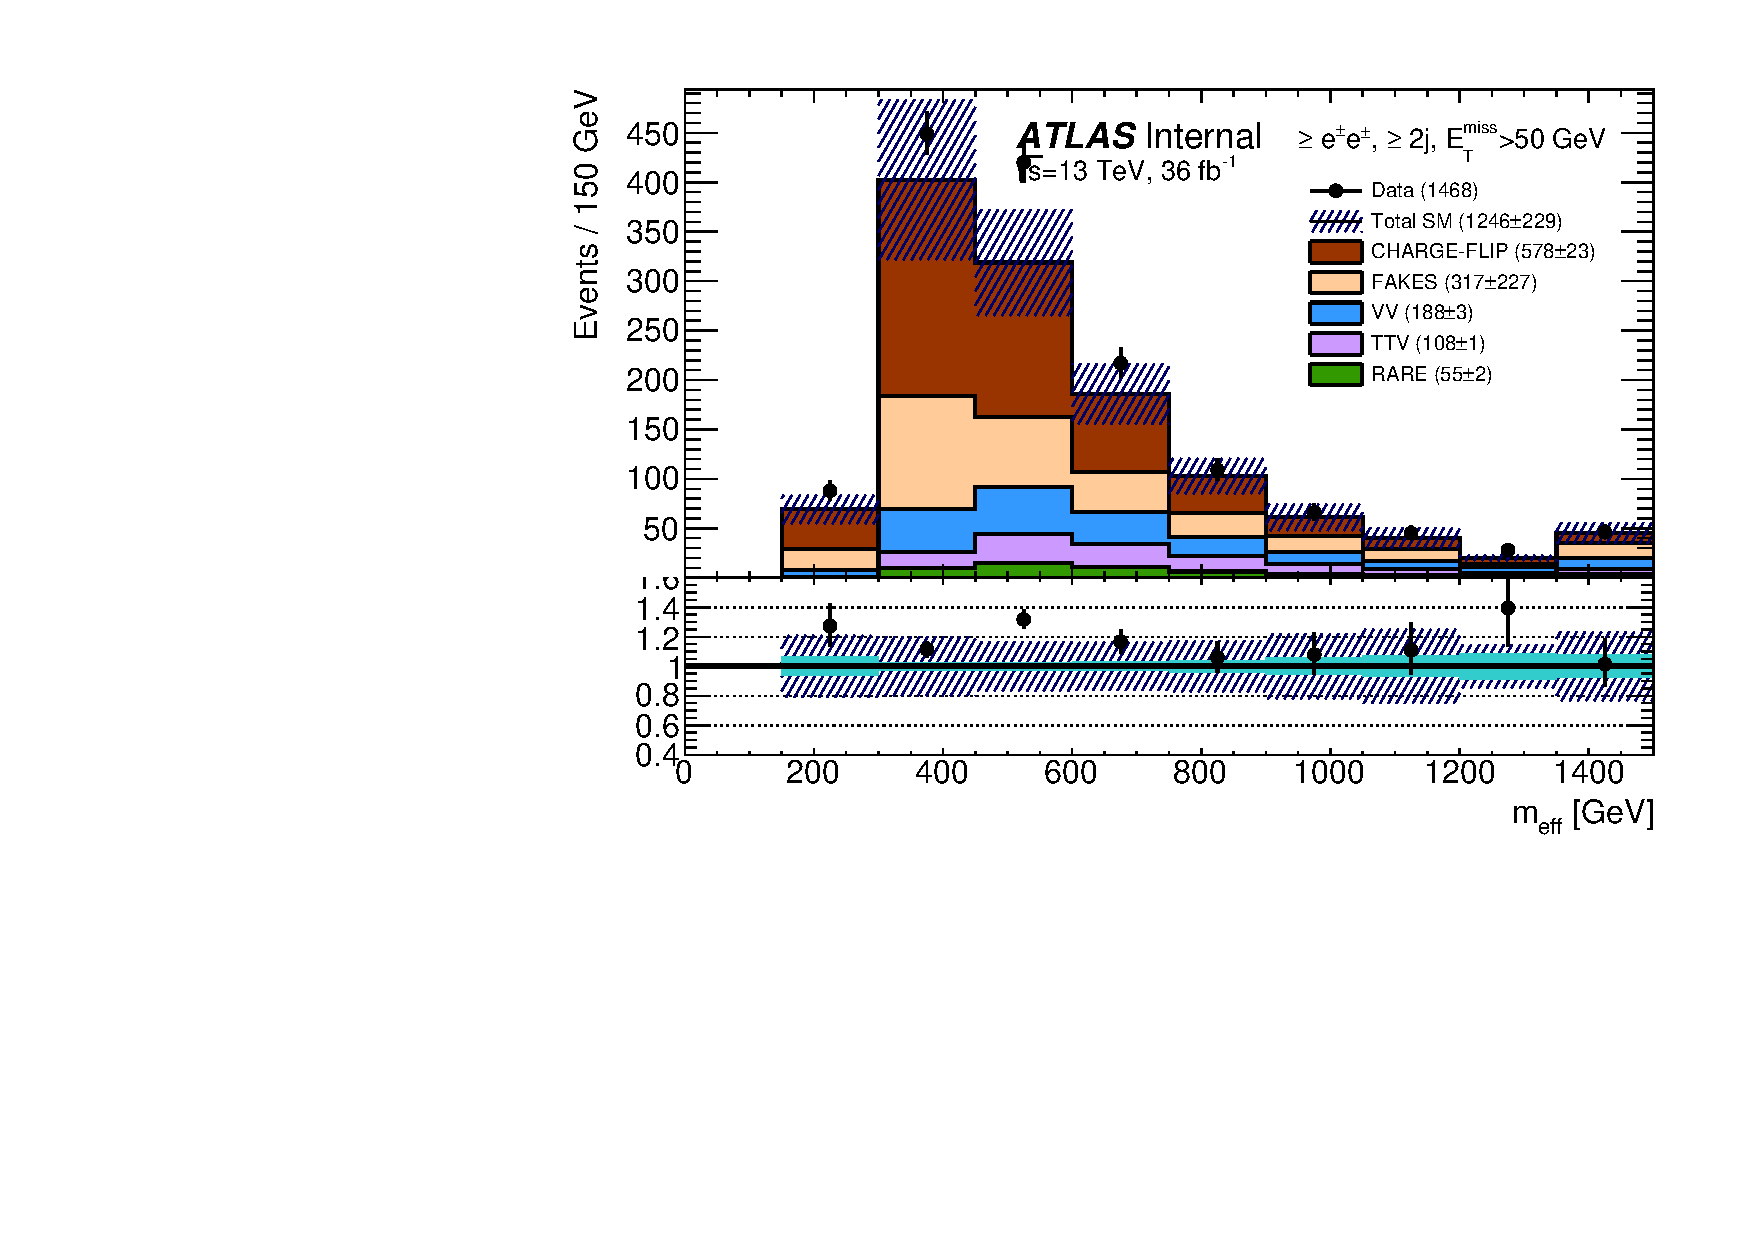
\includegraphics[width=\textwidth]{EE_2JMET50_meff}
\caption{Effective mass \meff}
\end{subfigure}
\begin{subfigure}[t]{0.48\textwidth}
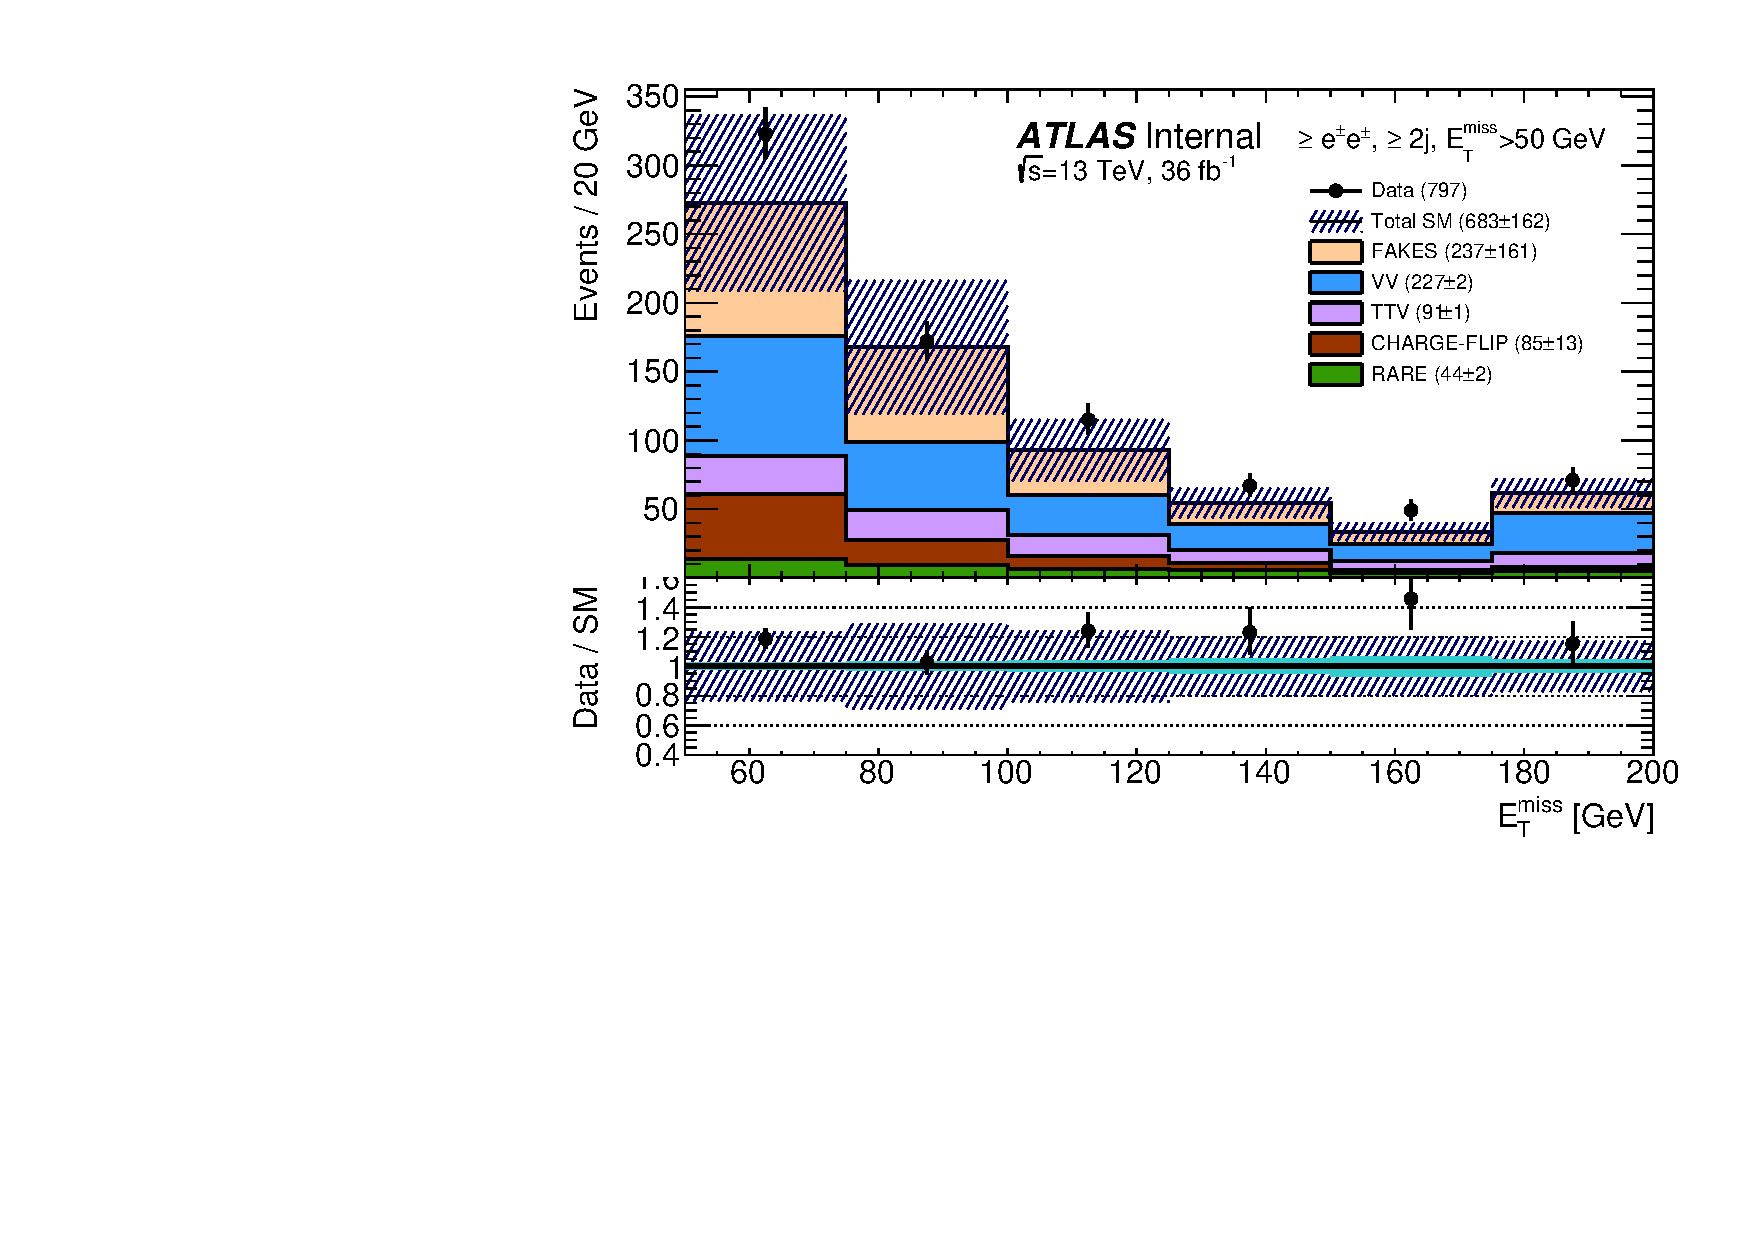
\includegraphics[width=\textwidth]{EE_2JMET50_met}
\caption{Missing transverse momentum \met}
\end{subfigure}
\begin{subfigure}[t]{0.48\textwidth}
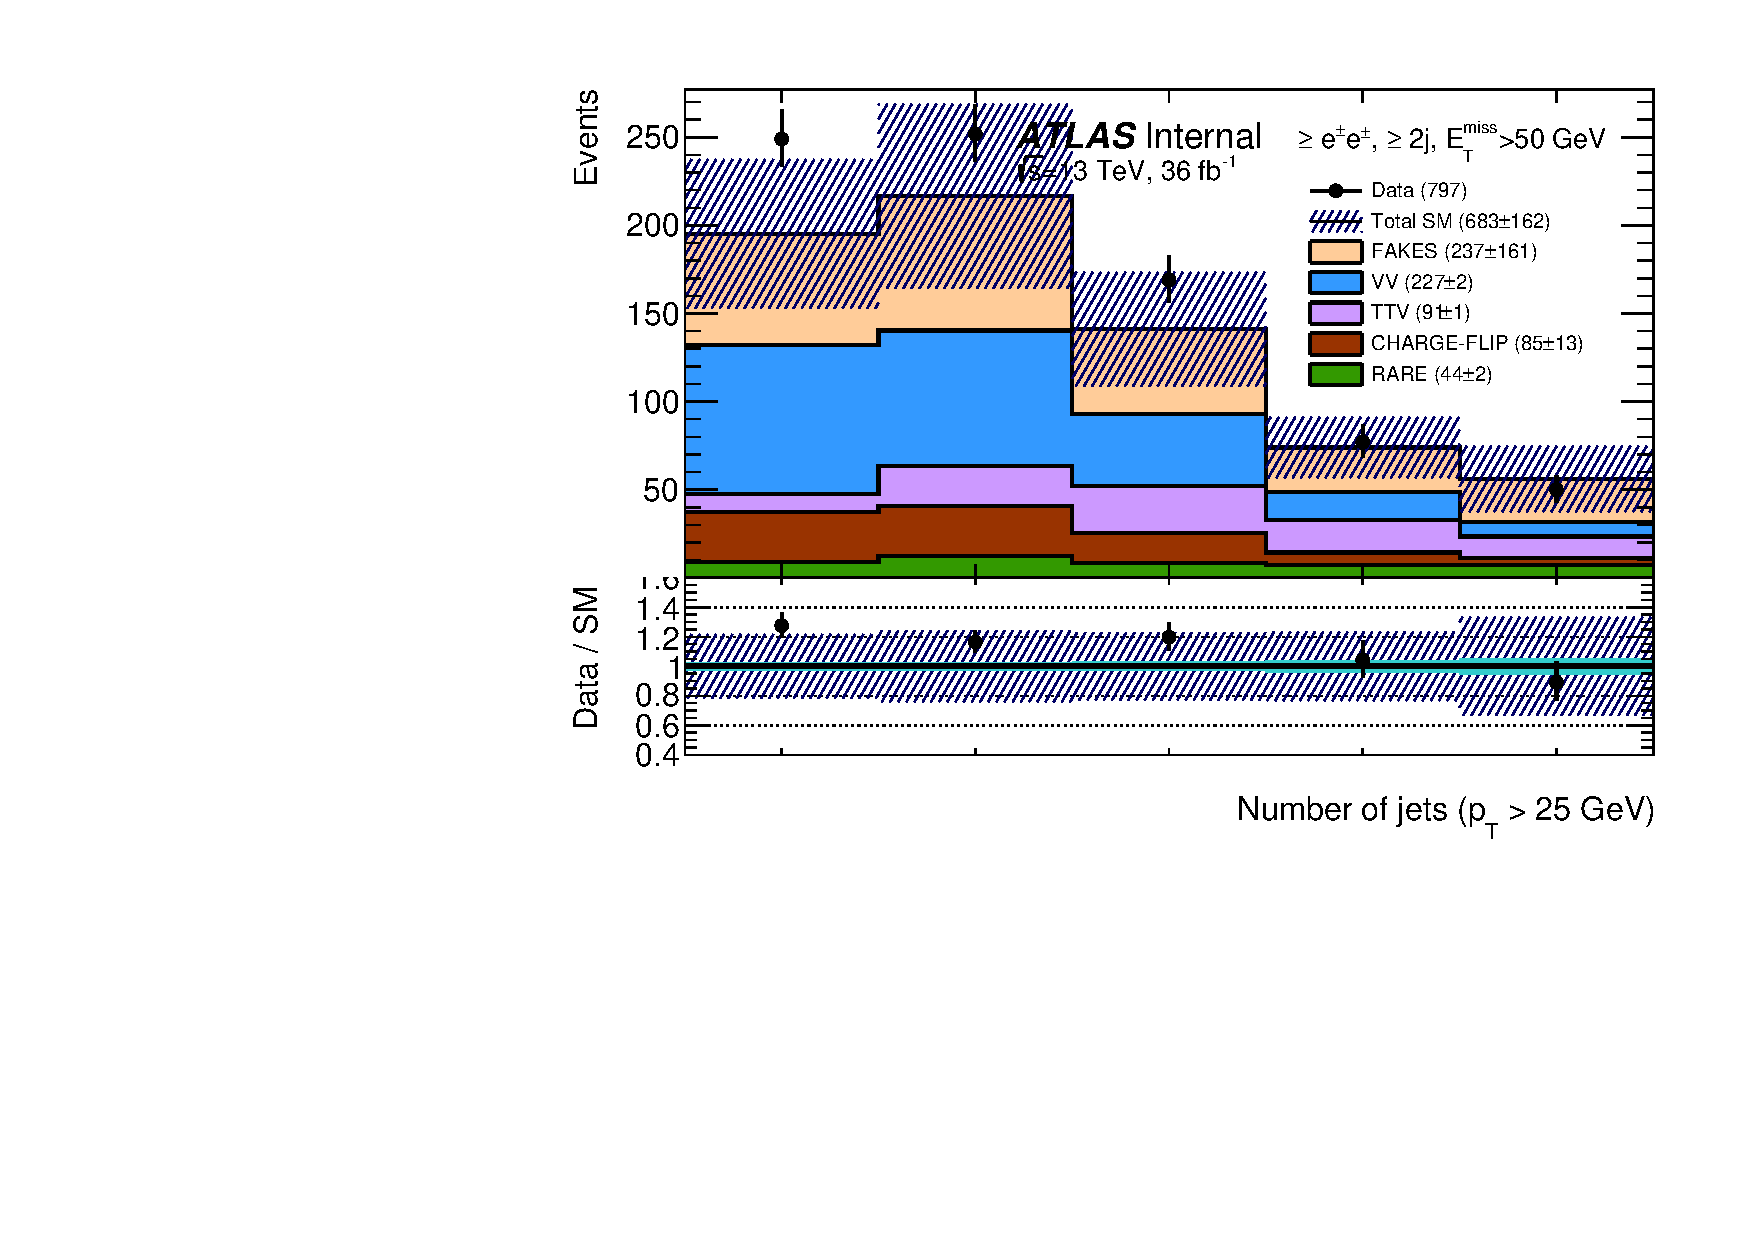
\includegraphics[width=\textwidth]{EE_2JMET50_njets25}
\caption{Number of jets ($\pt>25~\GeV$)}
\end{subfigure}
\begin{subfigure}[t]{0.48\textwidth}
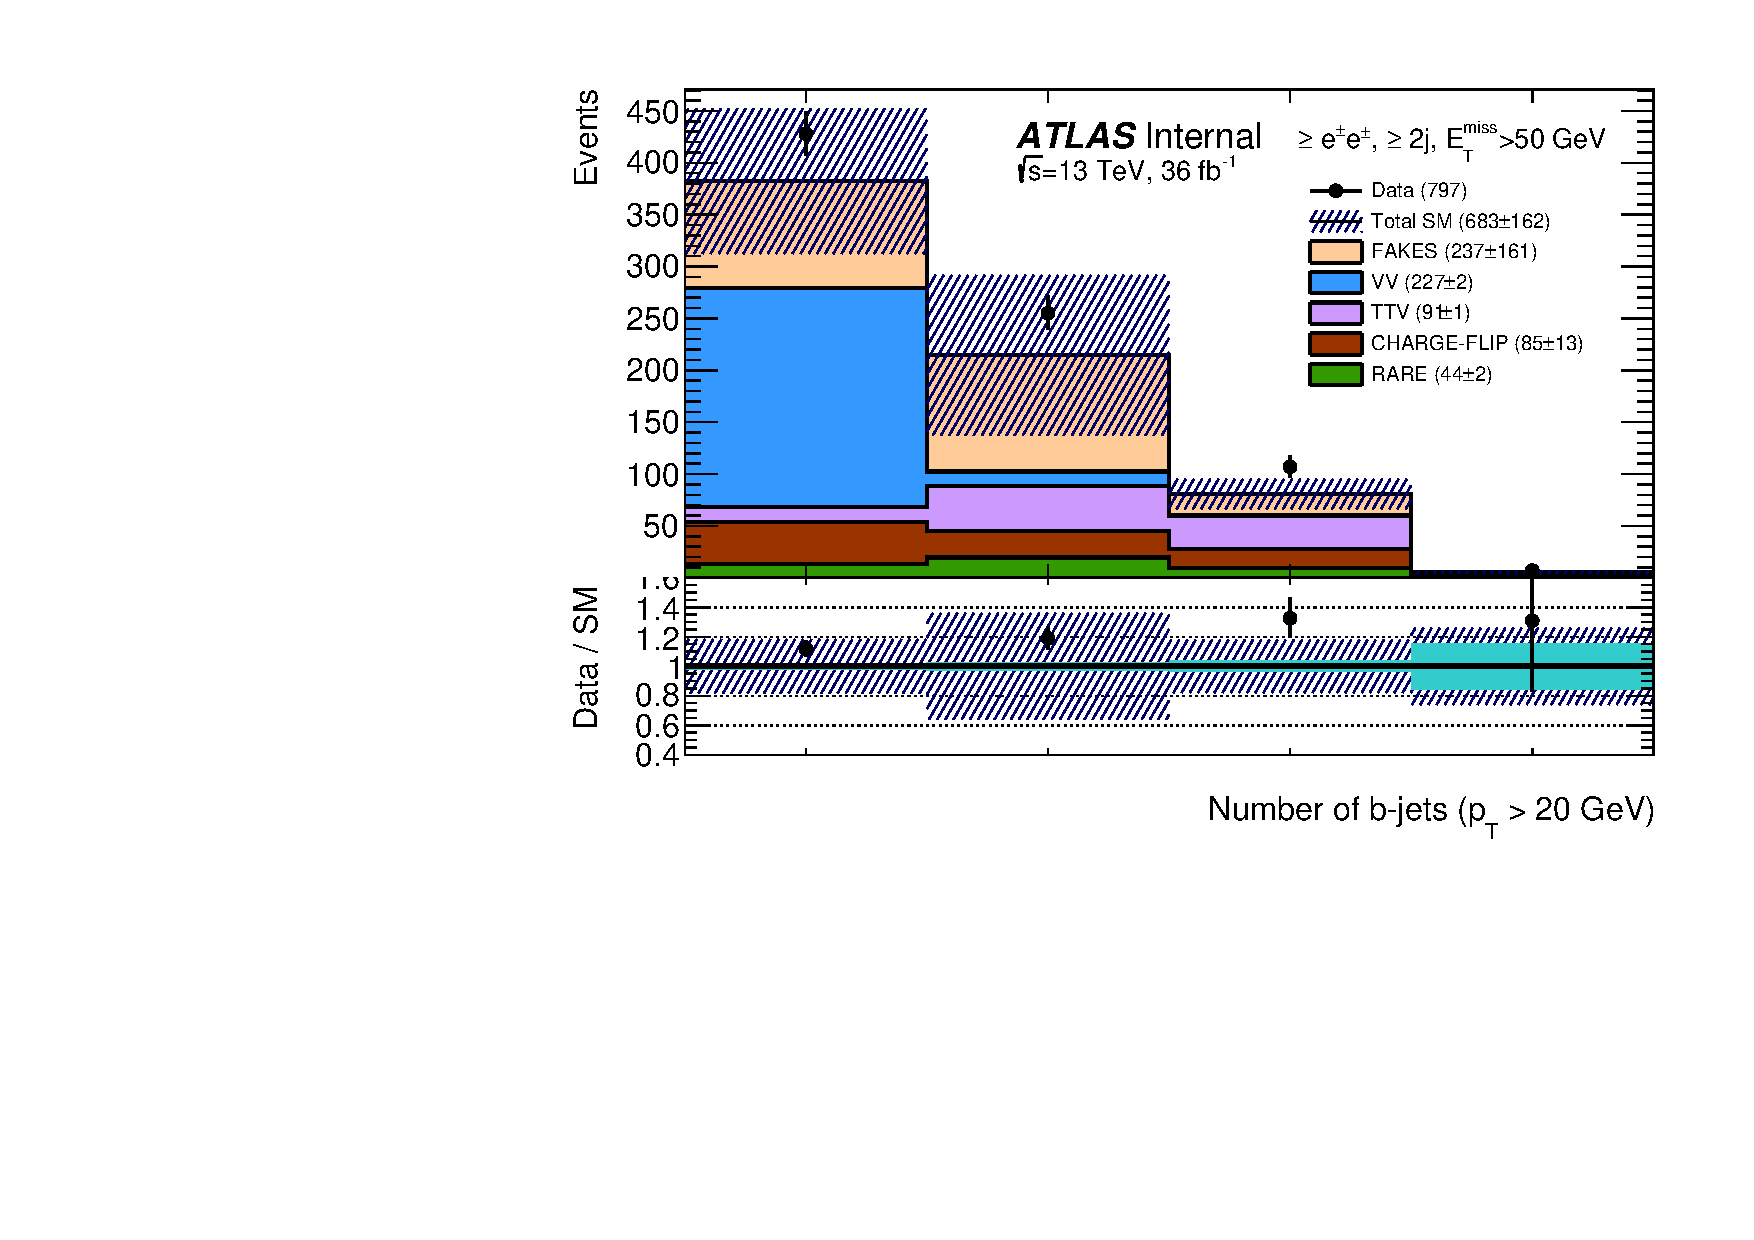
\includegraphics[width=\textwidth]{EE_2JMET50_nbjets}
\caption{Number of $b$-tagged jets ($\pt>20~\GeV$)}
\end{subfigure}
\begin{subfigure}[t]{0.48\textwidth}
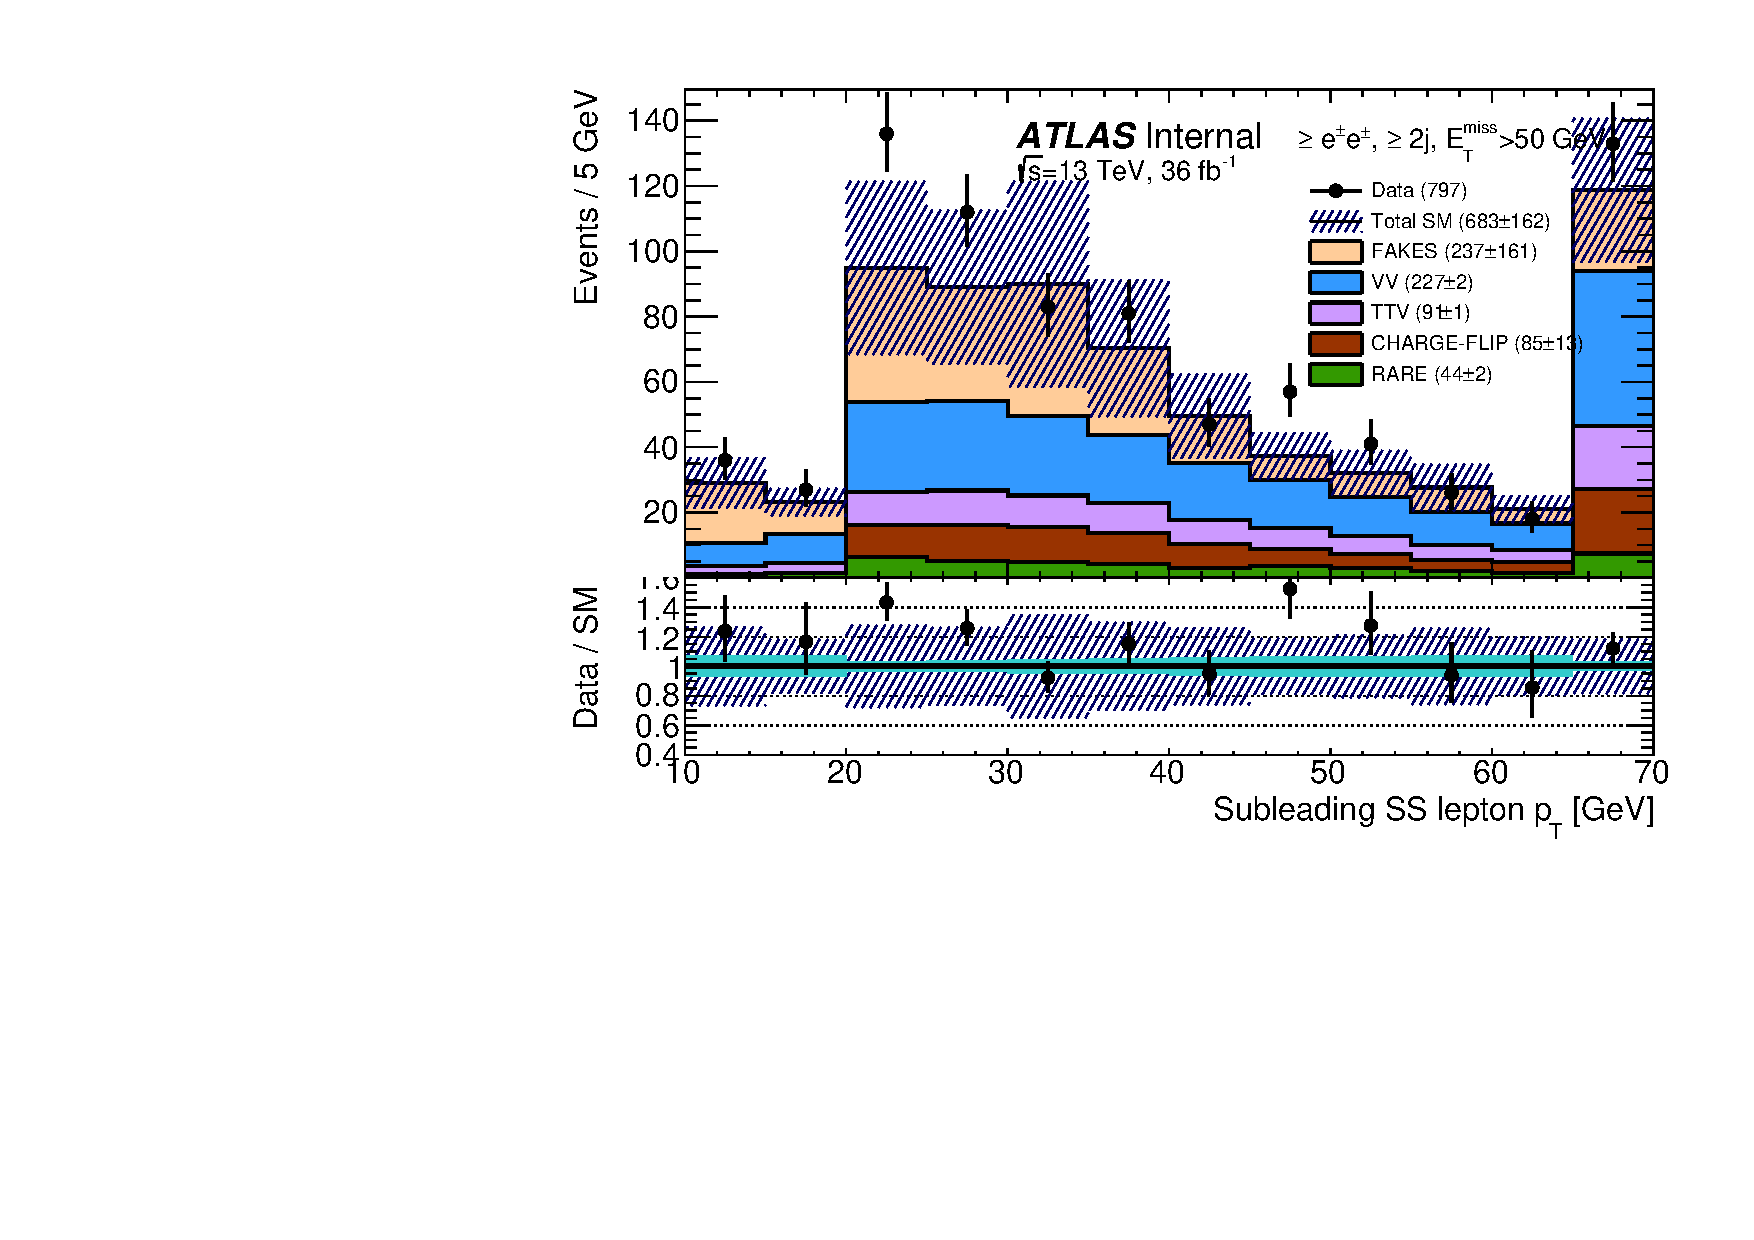
\includegraphics[width=\textwidth]{EE_2JMET50_subSS_Pt}
\caption{Subleading SS lepton \pt}
\end{subfigure}
\caption{Di-electron channel: comparisons between observed data (2015+2016, 36 \ifb) and expected SM+detector backgrounds 
for events with $\ge 2$ same-sign leptons ($\pt>20~\GeV$), $\met>50~\GeV$ and $\ge 2$ jets ($\pt>40~\GeV$). 
Uncertainties include statistical sources, as well as systematic uncertainties for the data-driven backgrounds; 
for illustration, statistical uncertainties alone are shown in the light-colored error bands in the ratio plots. 
Events belonging to any of the signal regions are rejected, both in data and MC. 
}
\label{fig:distributions_channelEE_2015}
\end{figure} 

\begin{figure}[t!]
\centering
\begin{subfigure}[t]{0.48\textwidth}
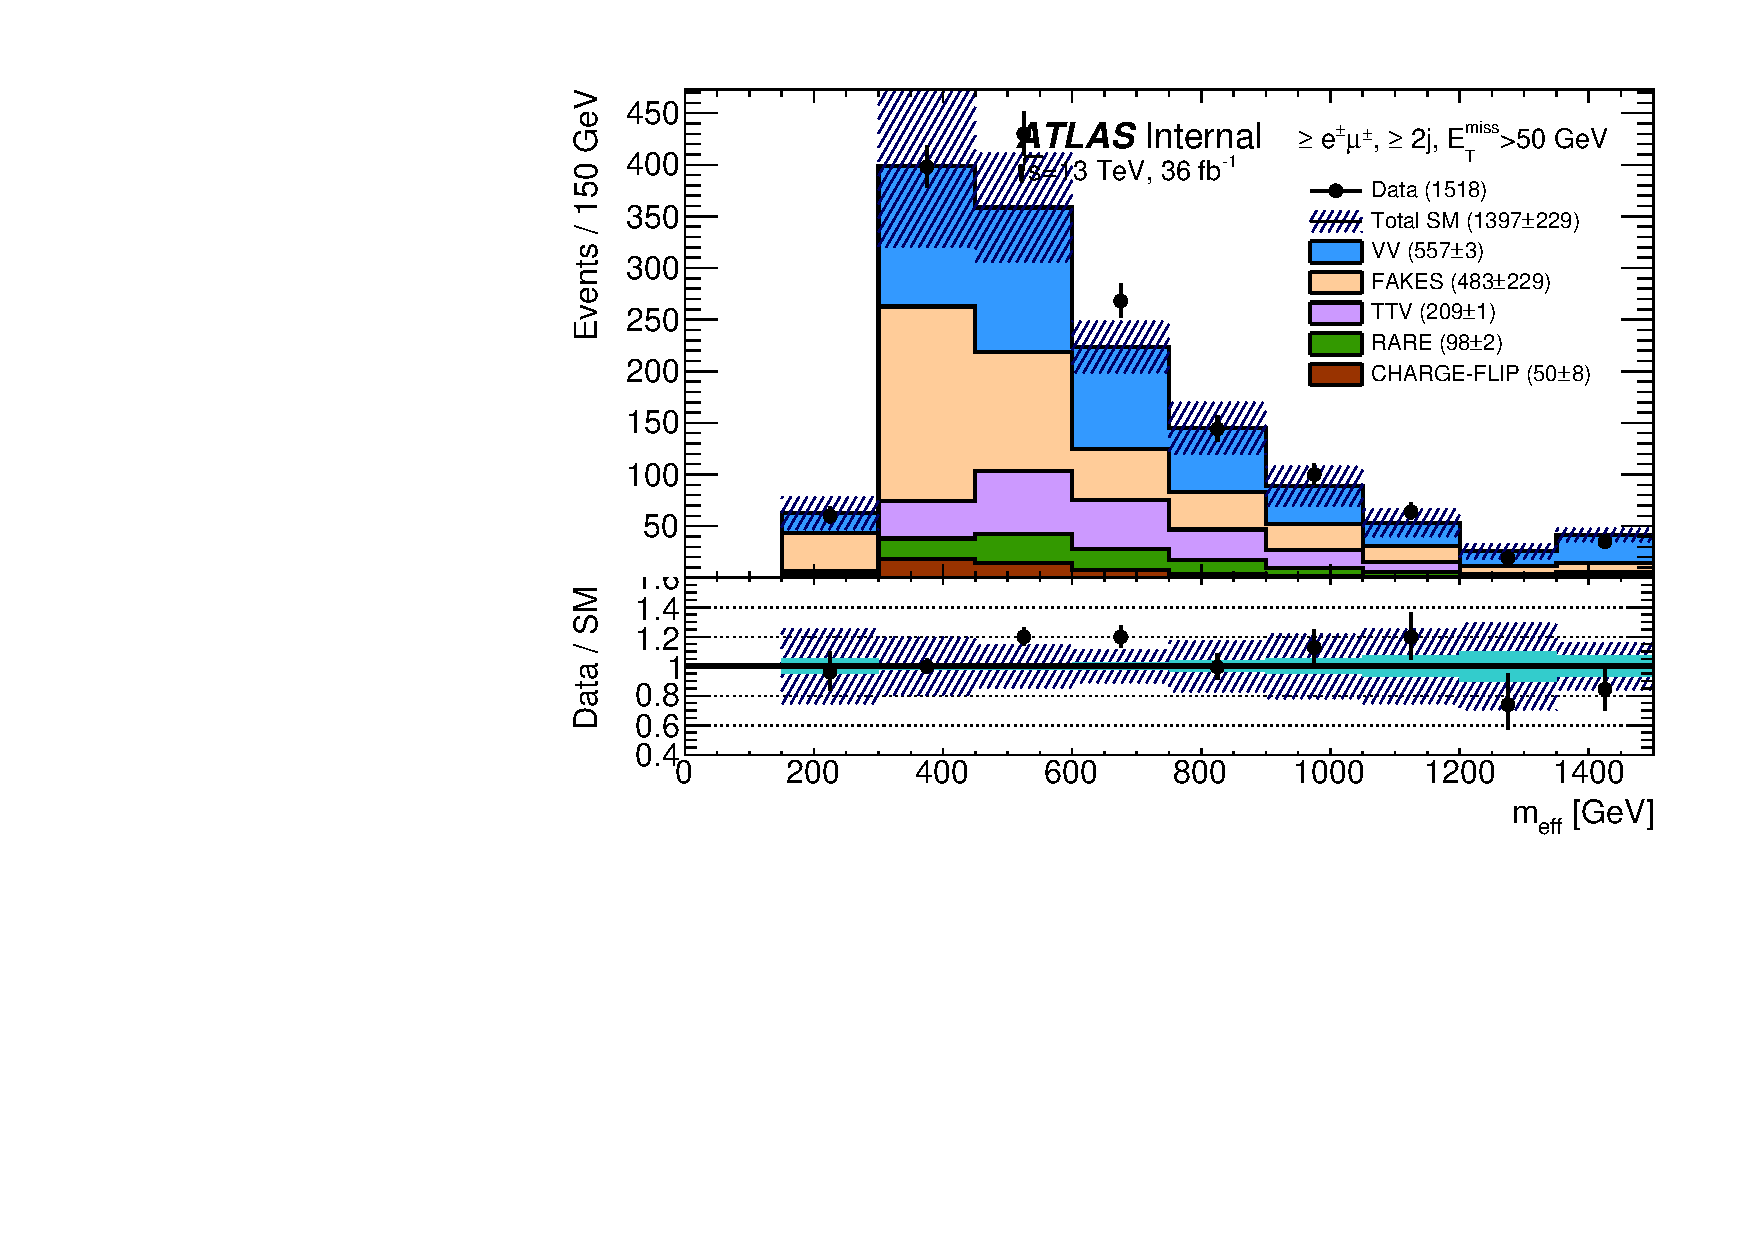
\includegraphics[width=\textwidth]{EM_2JMET50_meff}
\caption{Effective mass \meff}
\end{subfigure}
\begin{subfigure}[t]{0.48\textwidth}
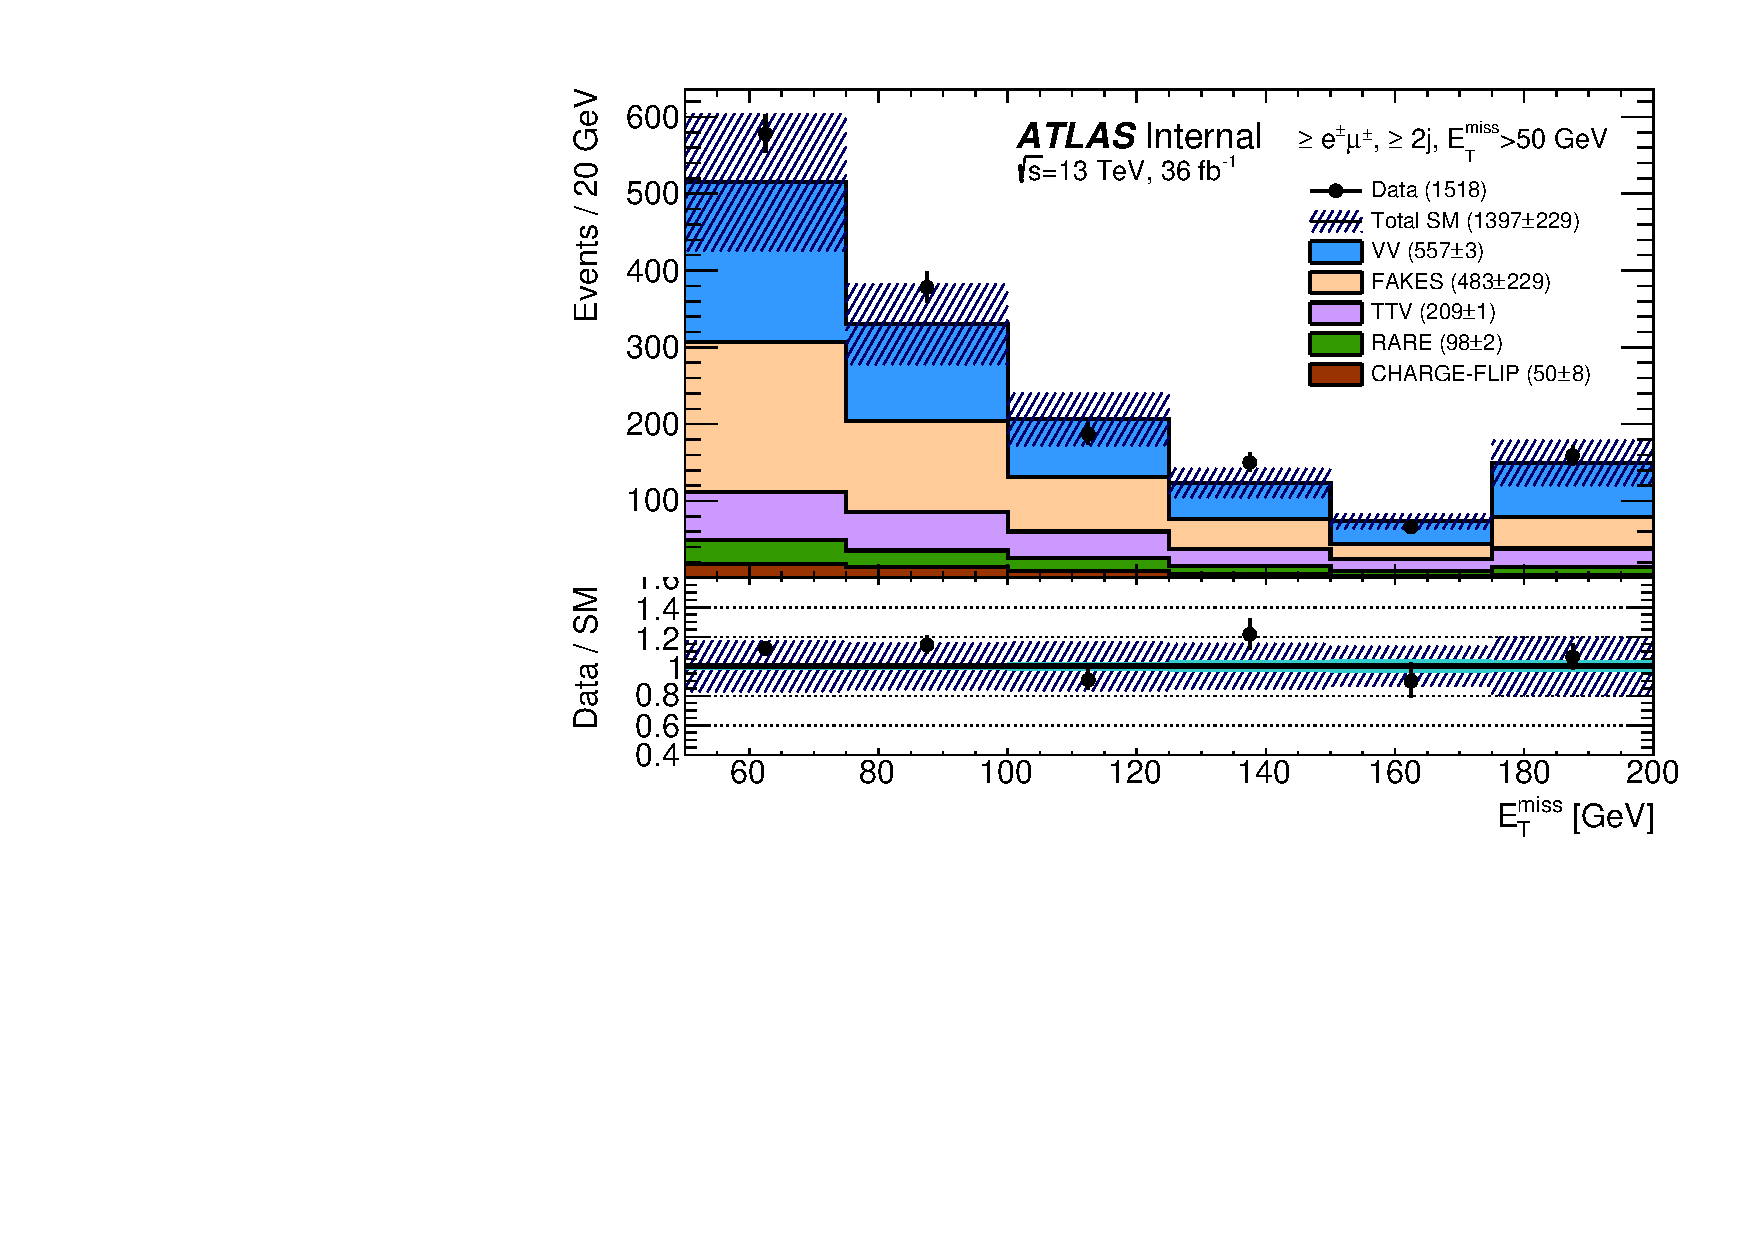
\includegraphics[width=\textwidth]{EM_2JMET50_met}
\caption{Missing transverse momentum \met}
\end{subfigure}
\begin{subfigure}[t]{0.48\textwidth}
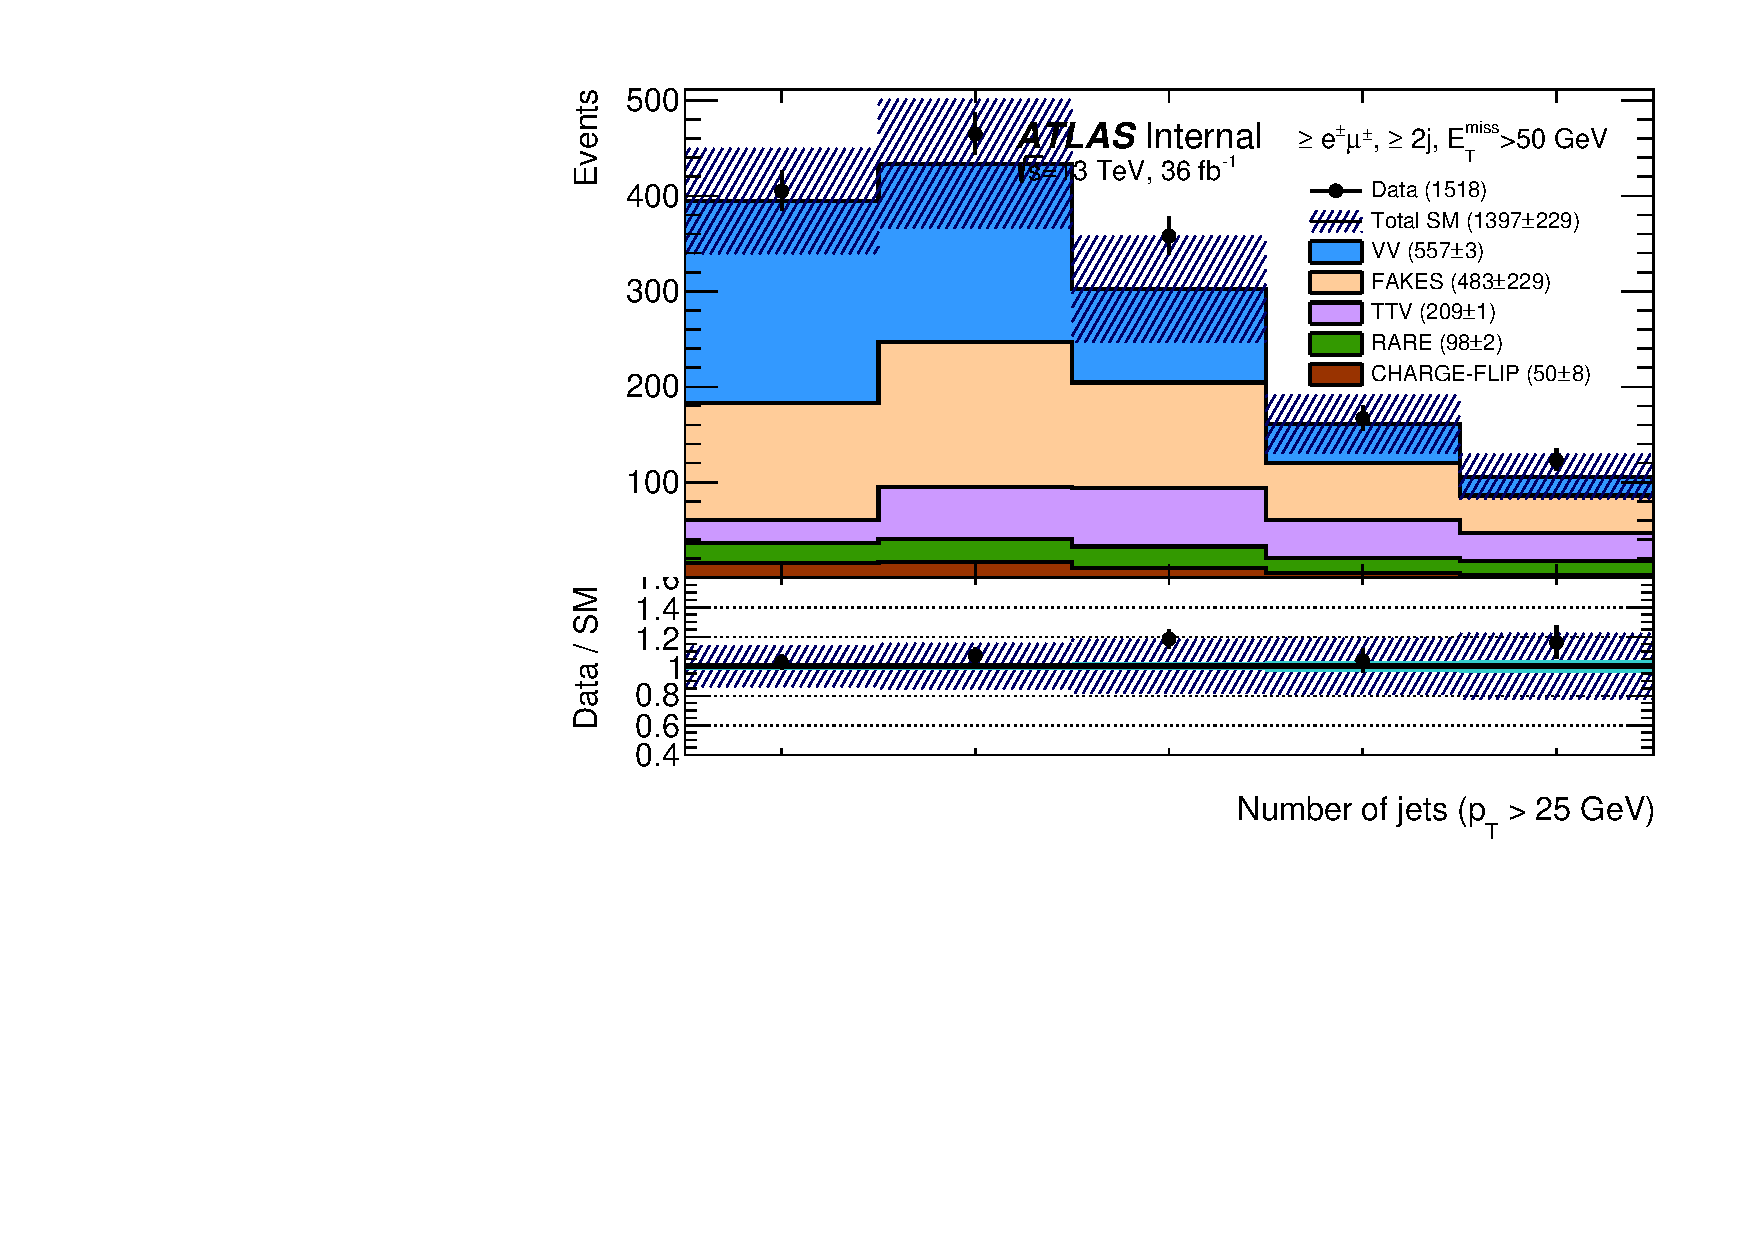
\includegraphics[width=\textwidth]{EM_2JMET50_njets25}
\caption{Number of jets ($\pt>25~\GeV$)}
\end{subfigure}
\begin{subfigure}[t]{0.48\textwidth}
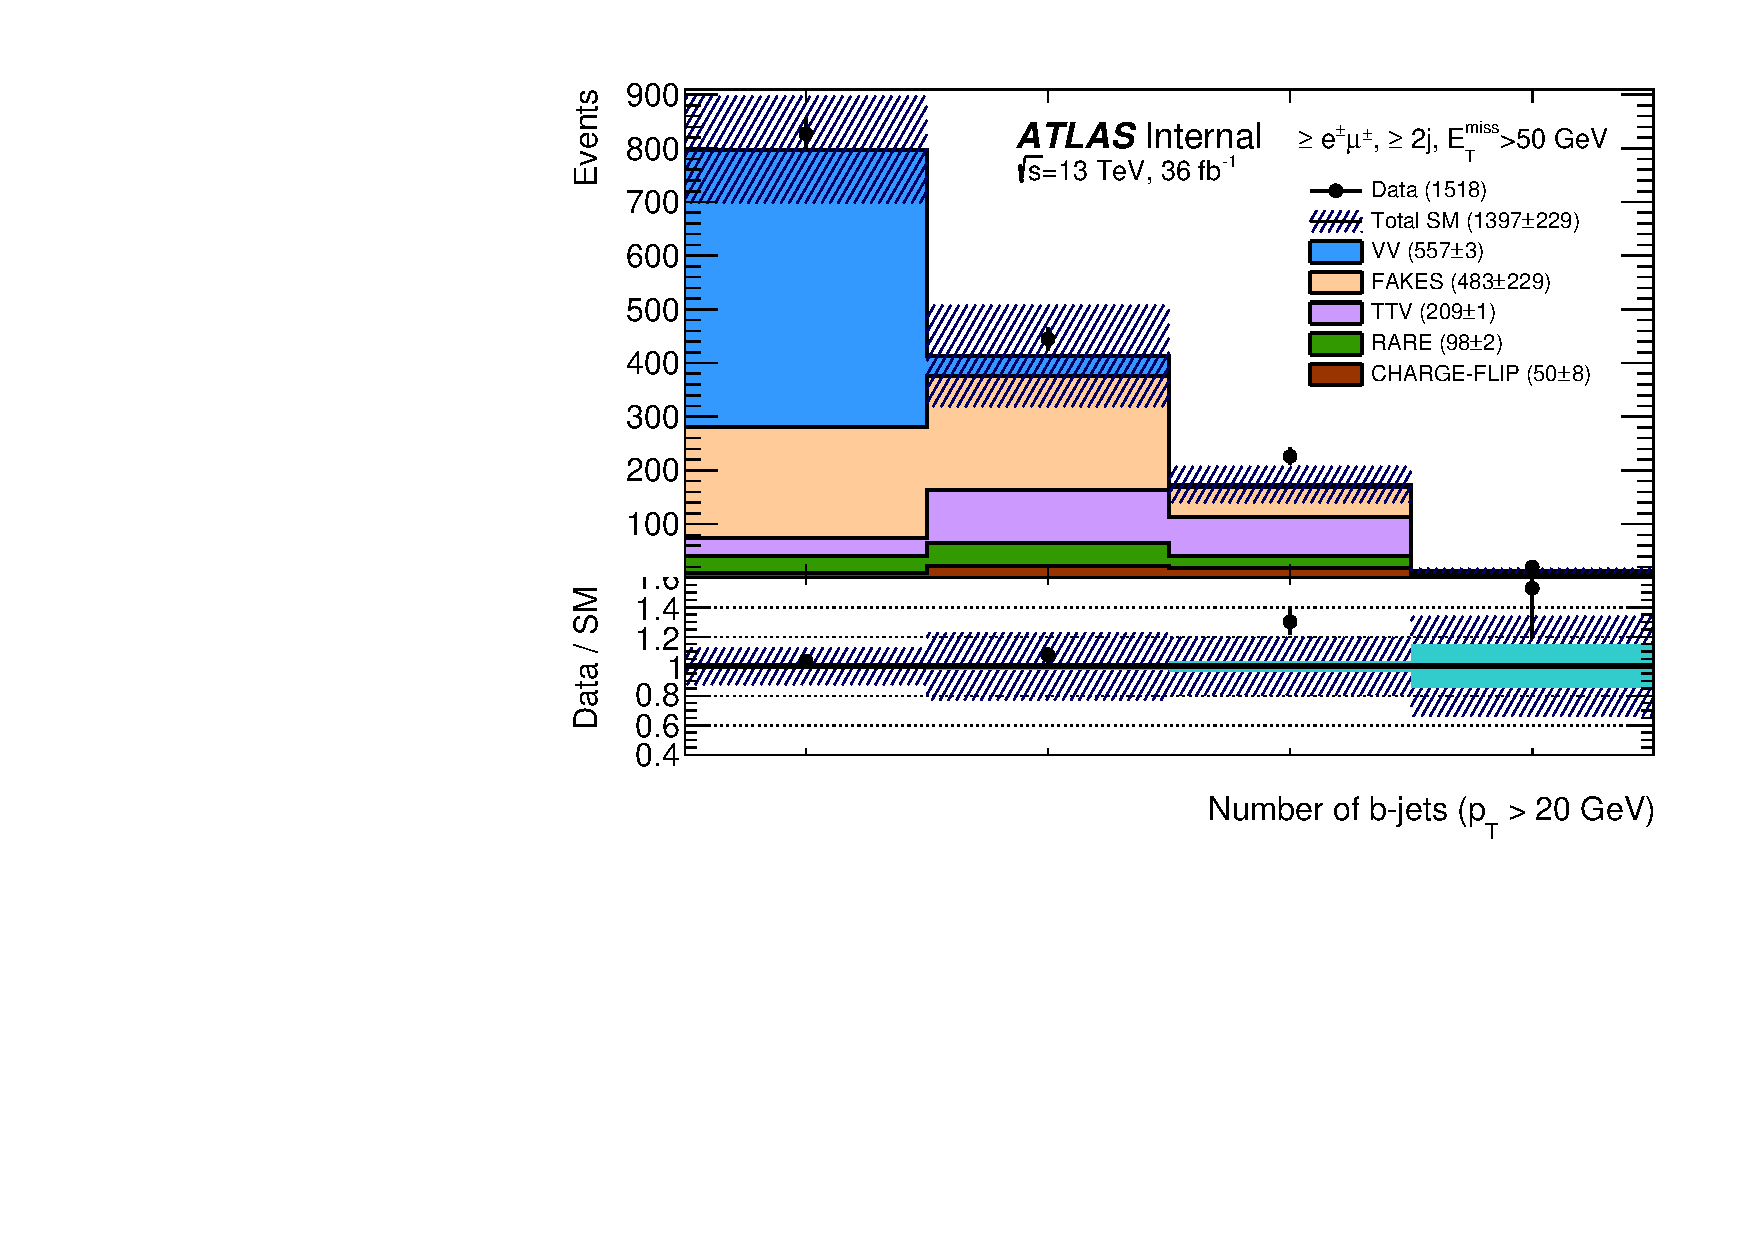
\includegraphics[width=\textwidth]{EM_2JMET50_nbjets}
\caption{Number of $b$-tagged jets ($\pt>20~\GeV$)}
\end{subfigure}
\begin{subfigure}[t]{0.48\textwidth}
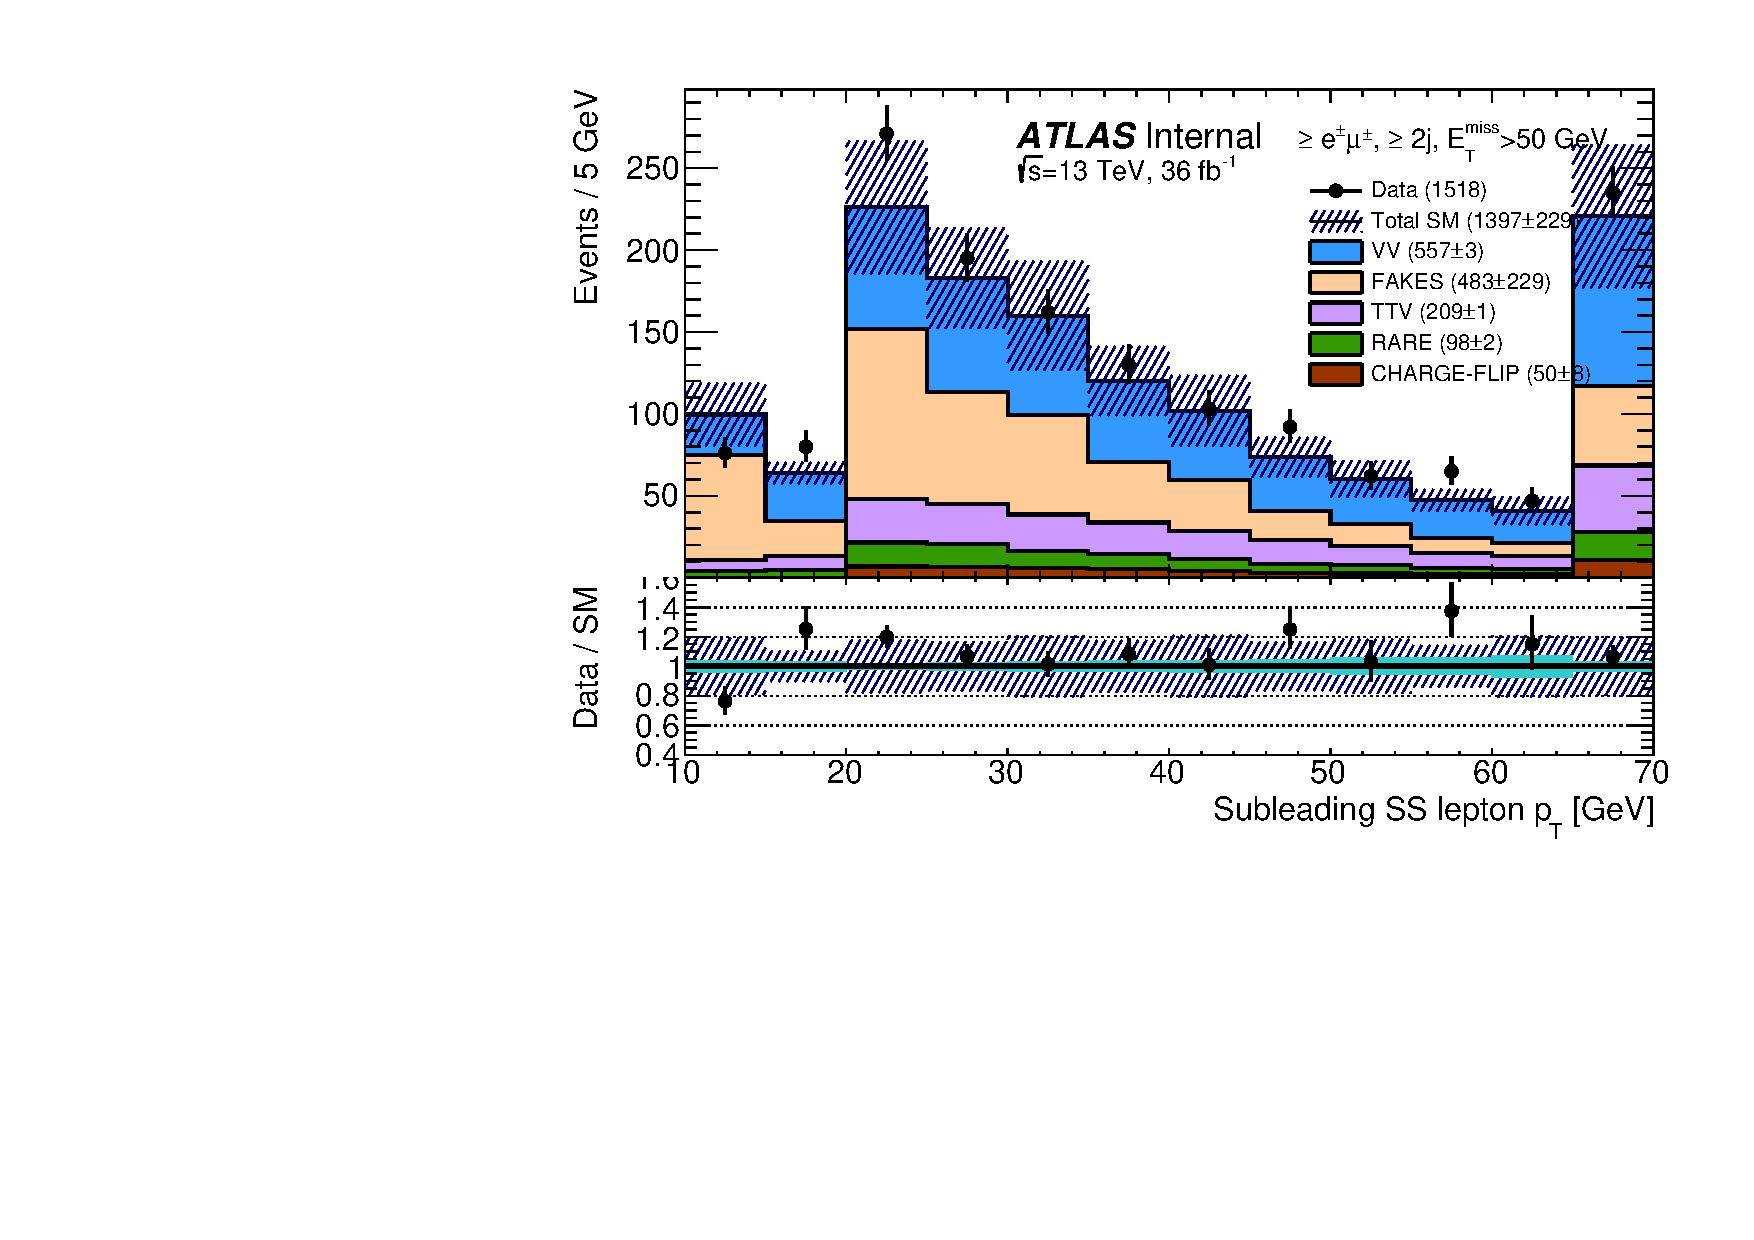
\includegraphics[width=\textwidth]{EM_2JMET50_subSS_Pt}
\caption{Subleading SS lepton \pt}
\end{subfigure}
\caption{Electron-muon channel: comparisons between observed data (2015+2016, 36 \ifb) and expected SM+detector backgrounds 
for events with $\ge 2$ same-sign leptons ($\pt>20~\GeV$), $\met>50~\GeV$ and $\ge 2$ jets ($\pt>40~\GeV$). 
Uncertainties include statistical sources, as well as systematic uncertainties for the data-driven backgrounds; 
for illustration, statistical uncertainties alone are shown in the light-colored error bands in the ratio plots. 
Events belonging to any of the signal regions are rejected, both in data and MC.  
}
\label{fig:distributions_channelEM_2015}
\end{figure} 

\begin{figure}[t!]
\centering
\begin{subfigure}[t]{0.48\textwidth}
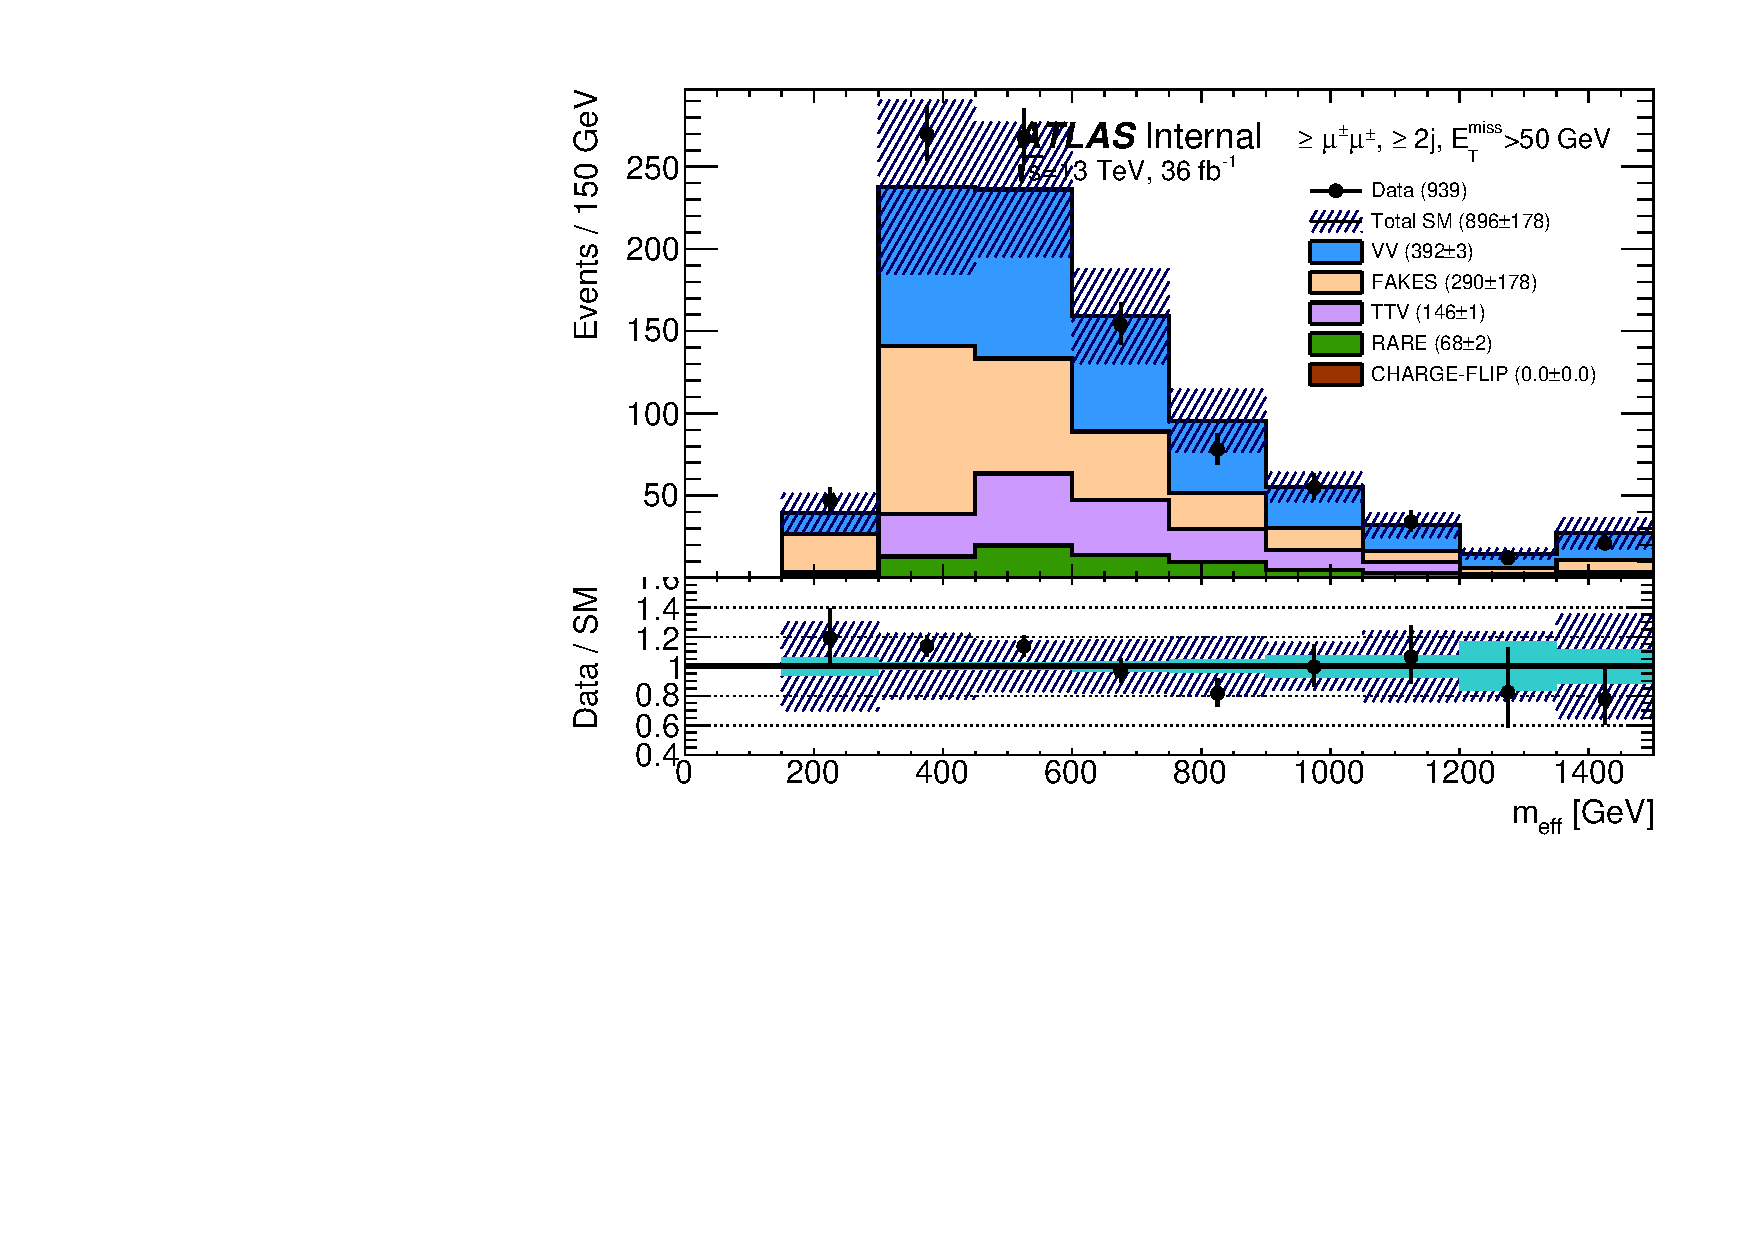
\includegraphics[width=\textwidth]{MM_2JMET50_meff}
\caption{Effective mass \meff}
\end{subfigure}
\begin{subfigure}[t]{0.48\textwidth}
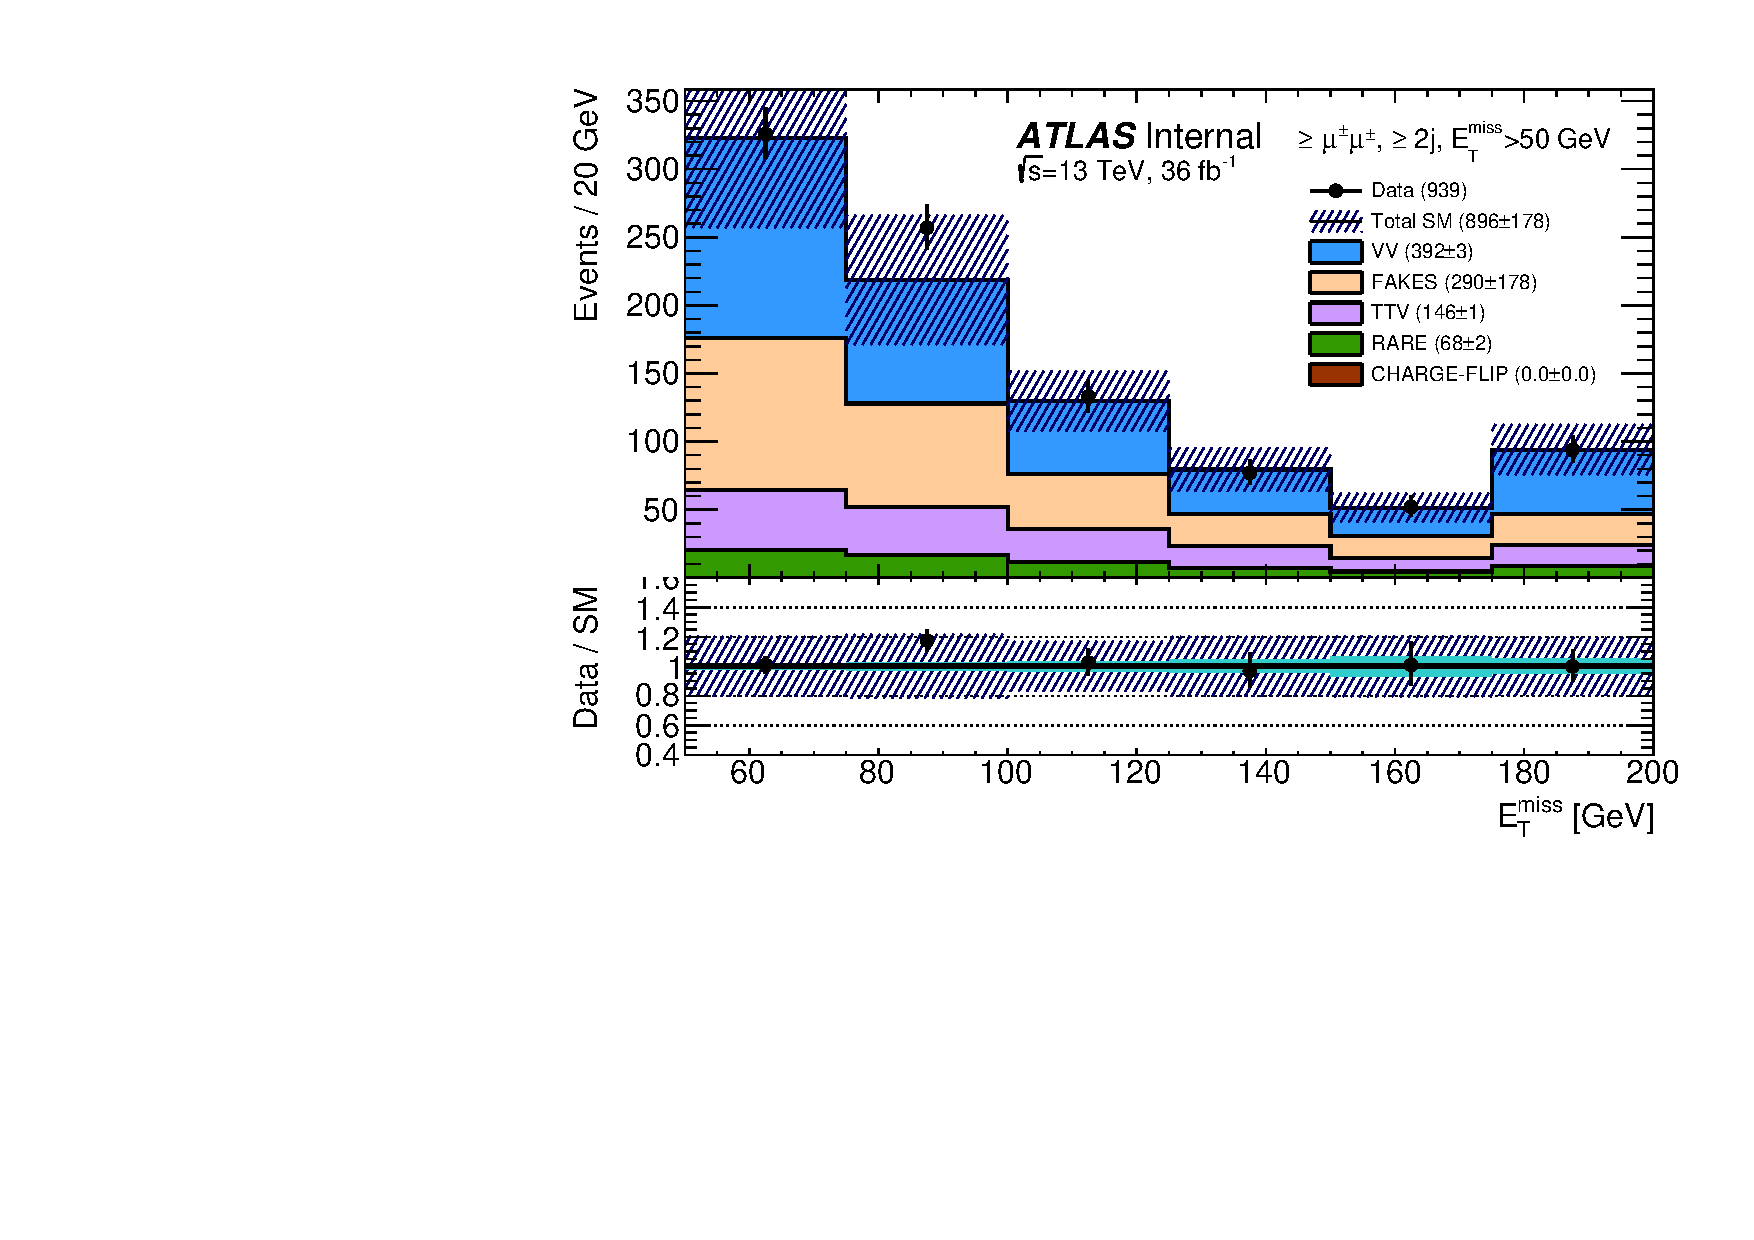
\includegraphics[width=\textwidth]{MM_2JMET50_met}
\caption{Missing transverse momentum \met}
\end{subfigure}
\begin{subfigure}[t]{0.48\textwidth}
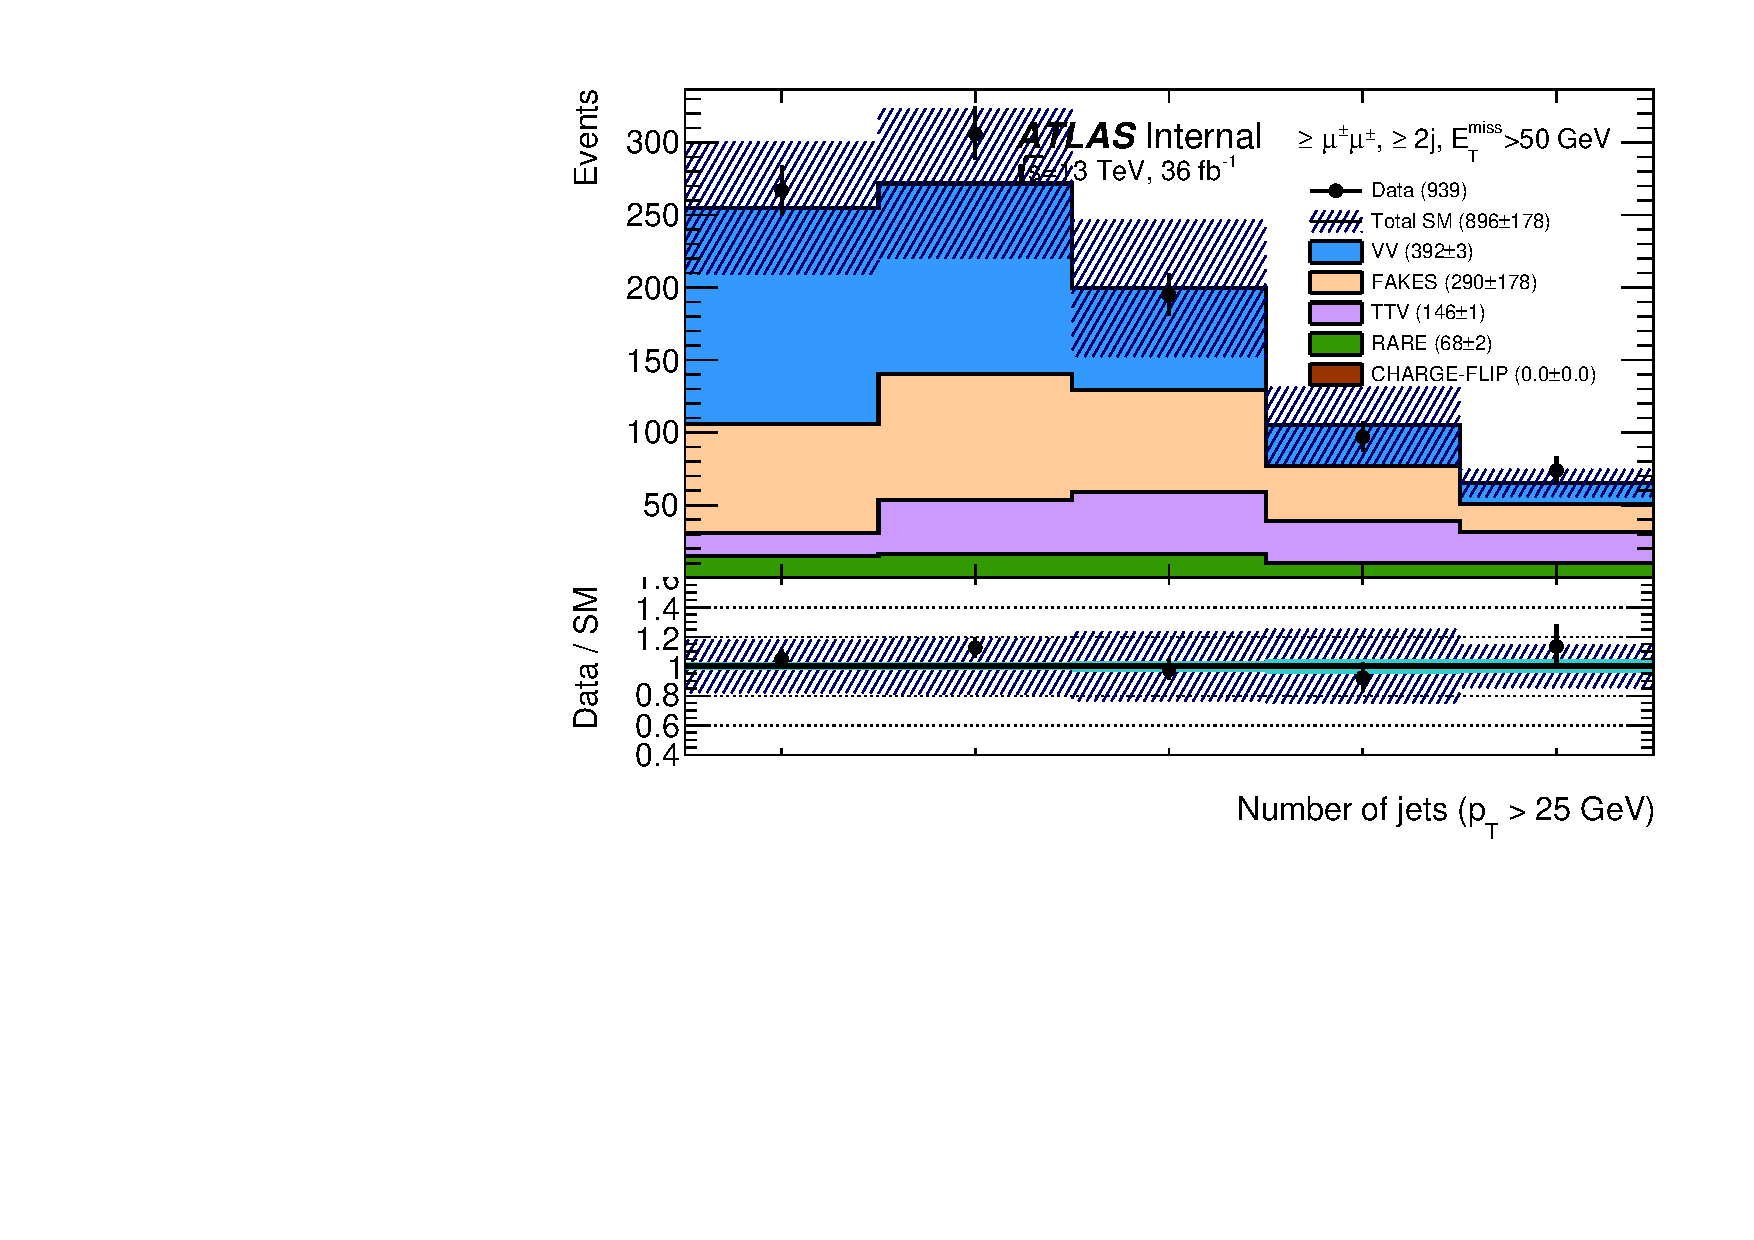
\includegraphics[width=\textwidth]{MM_2JMET50_njets25}
\caption{Number of jets ($\pt>25~\GeV$)}
\end{subfigure}
\begin{subfigure}[t]{0.48\textwidth}
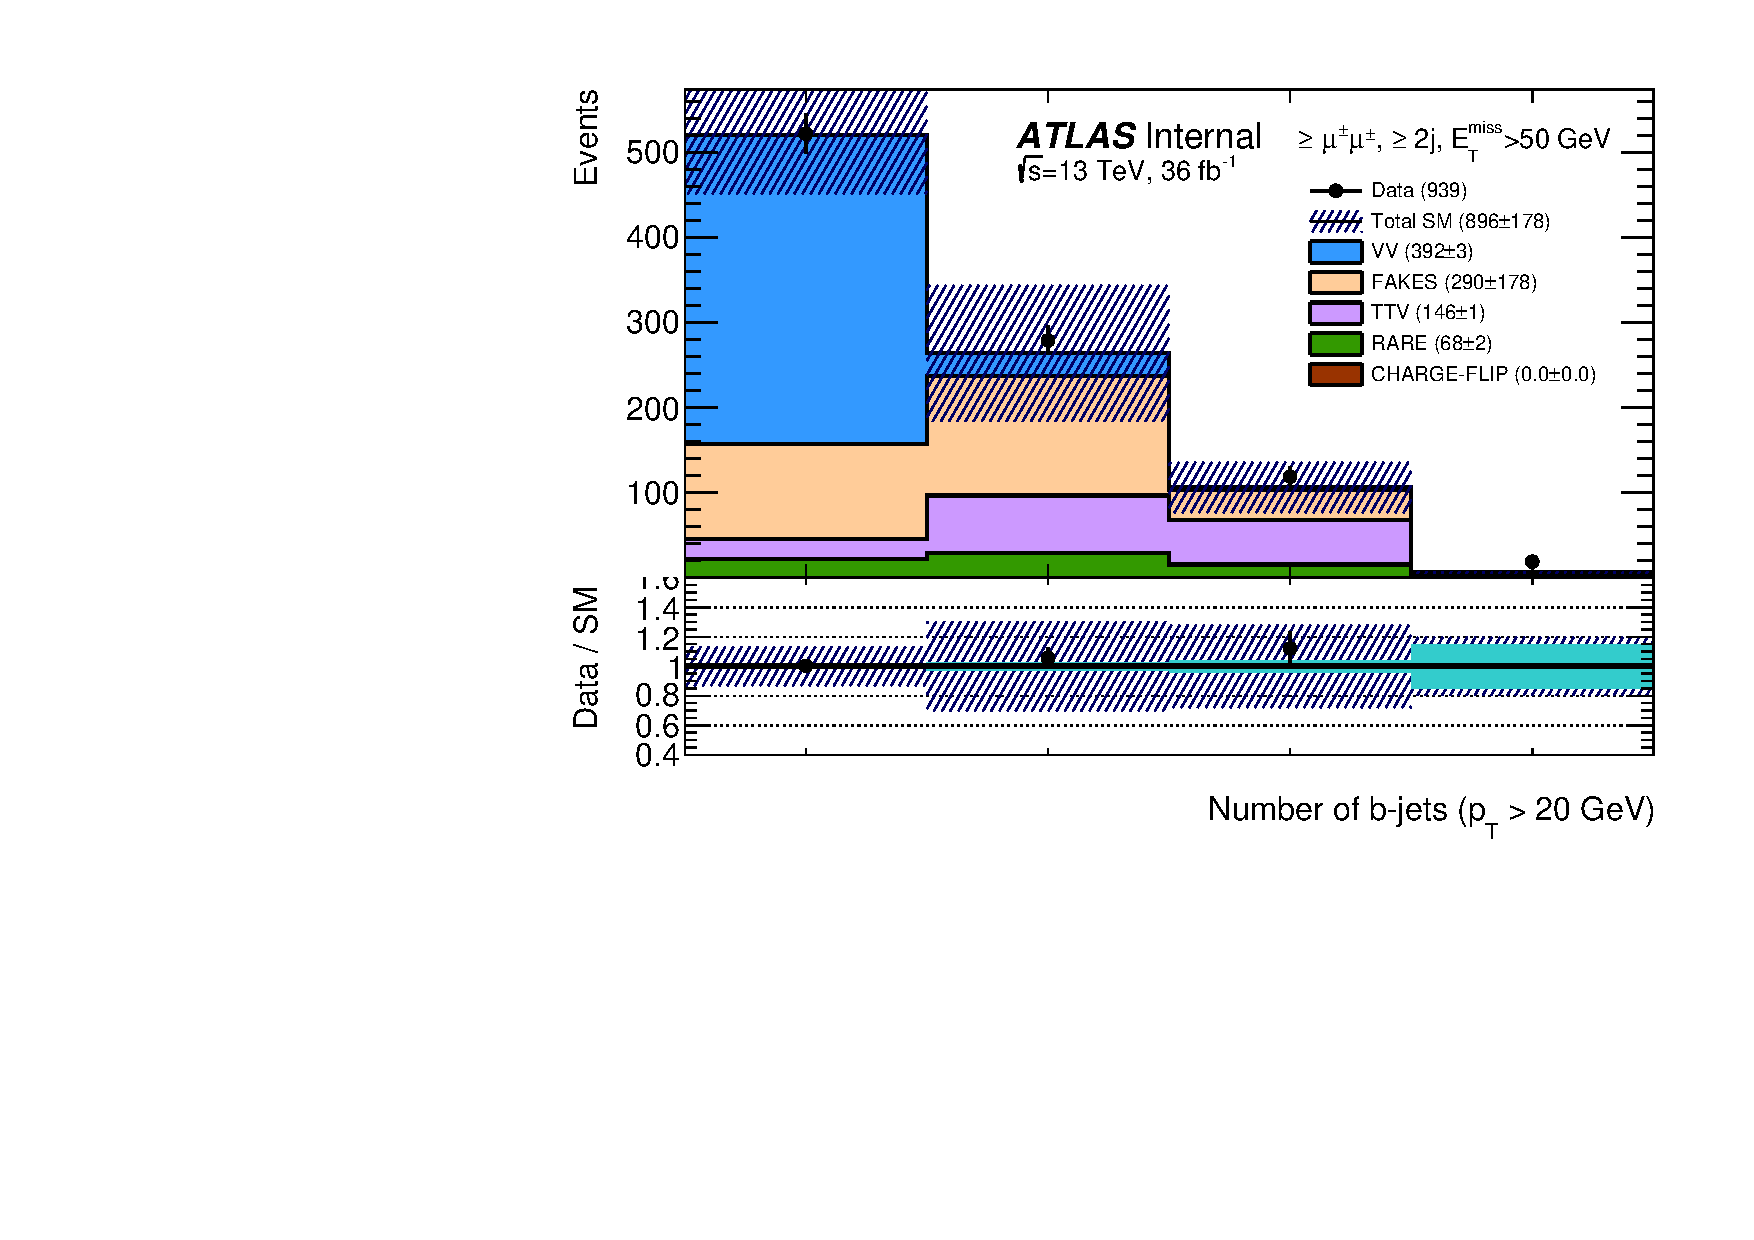
\includegraphics[width=\textwidth]{MM_2JMET50_nbjets}
\caption{Number of $b$-tagged jets ($\pt>20~\GeV$)}
\end{subfigure}
\begin{subfigure}[t]{0.48\textwidth}
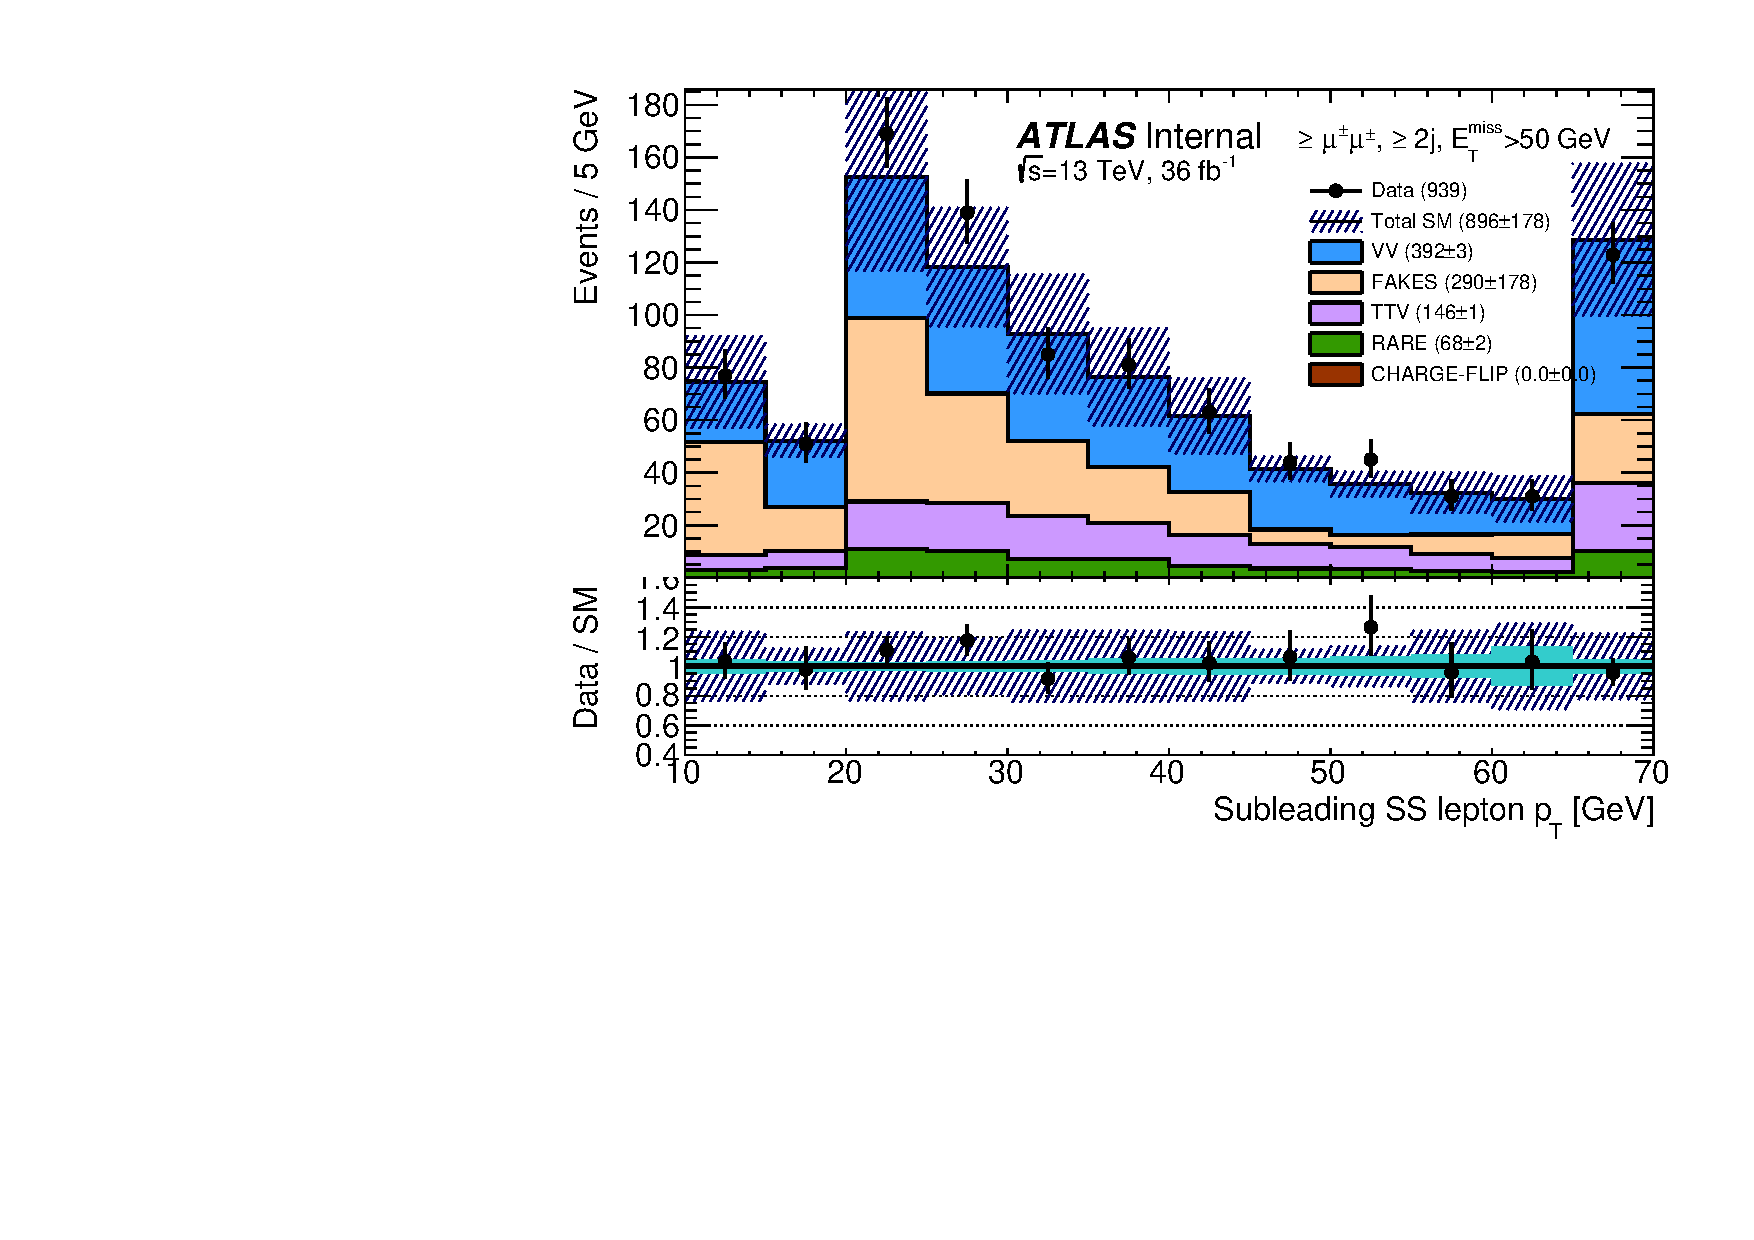
\includegraphics[width=\textwidth]{MM_2JMET50_subSS_Pt}
\caption{Subleading SS lepton \pt}
\end{subfigure}
\caption{Di-muon channel: comparisons between observed data (2015+2016, 36 \ifb) and expected SM+detector backgrounds 
for events with $\ge 2$ same-sign leptons ($\pt>20~\GeV$), $\met>50~\GeV$ and $\ge 2$ jets ($\pt>40~\GeV$). 
Uncertainties include statistical sources, as well as systematic uncertainties for the data-driven backgrounds; 
for illustration, statistical uncertainties alone are shown in the light-colored error bands in the ratio plots. 
Events belonging to any of the signal regions are rejected, both in data and MC.  
}
\label{fig:distributions_channelMM_2015}
\end{figure} 

\begin{figure}[t!]
\centering
\begin{subfigure}[t]{0.48\textwidth}
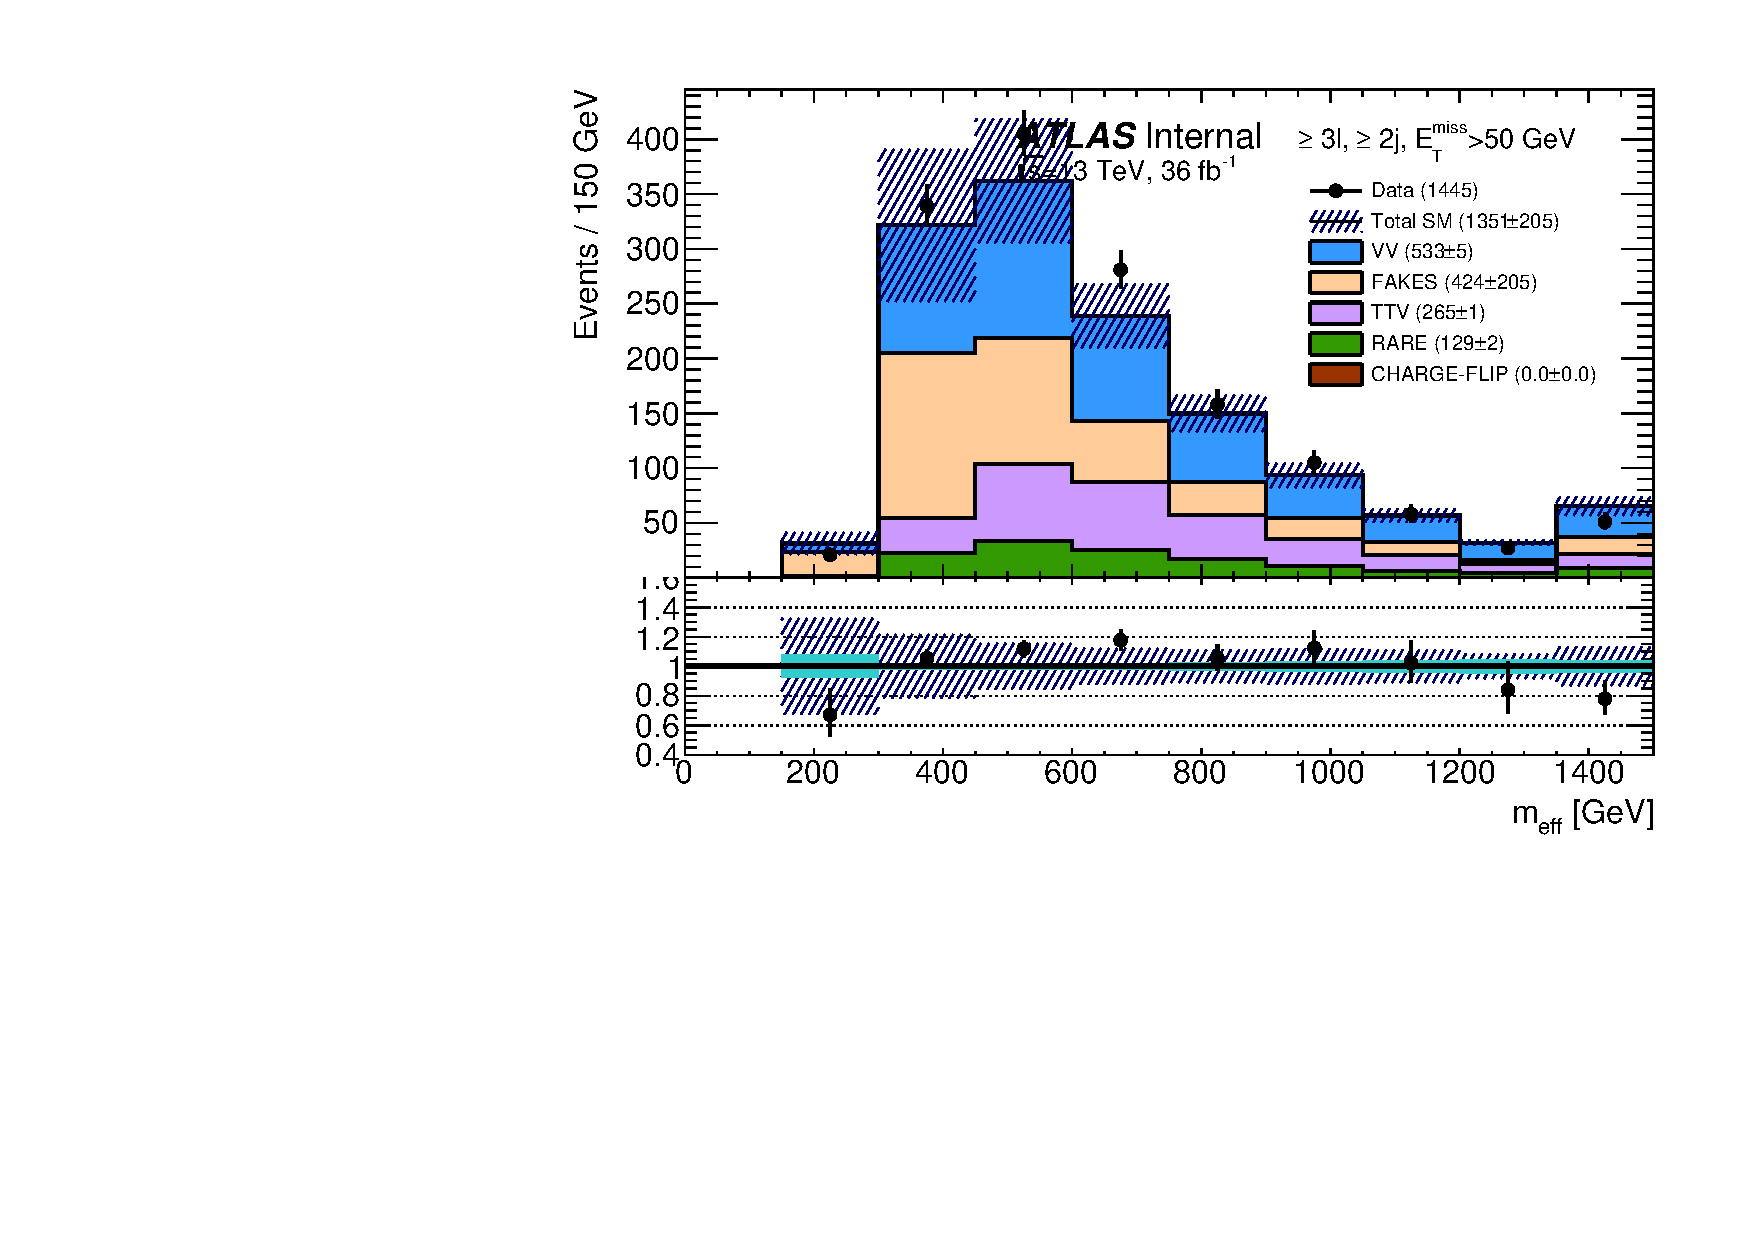
\includegraphics[width=\textwidth]{TRILEP_2JMET50_meff}
\caption{Effective mass \meff}
\end{subfigure}
\begin{subfigure}[t]{0.48\textwidth}
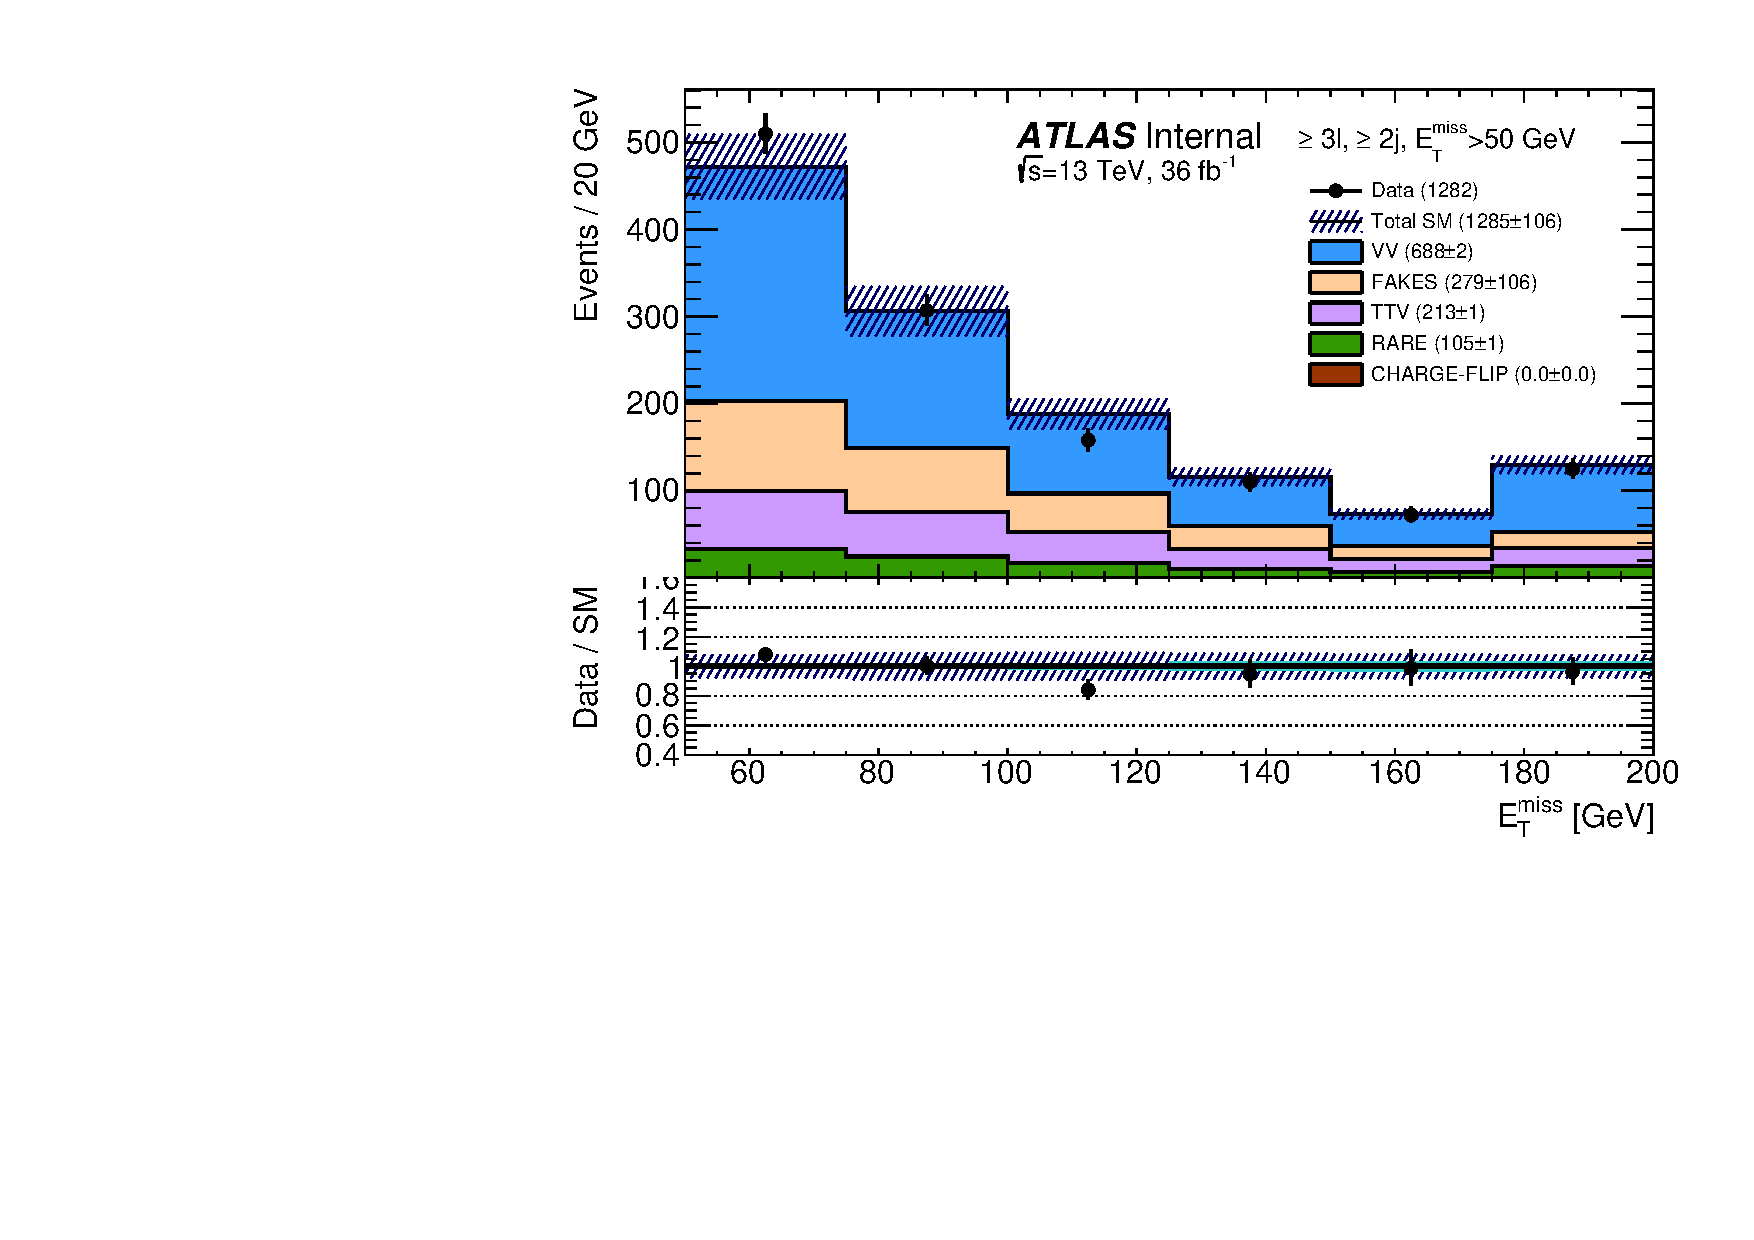
\includegraphics[width=\textwidth]{TRILEP_2JMET50_met}
\caption{Missing transverse momentum \met}
\end{subfigure}
\begin{subfigure}[t]{0.48\textwidth}
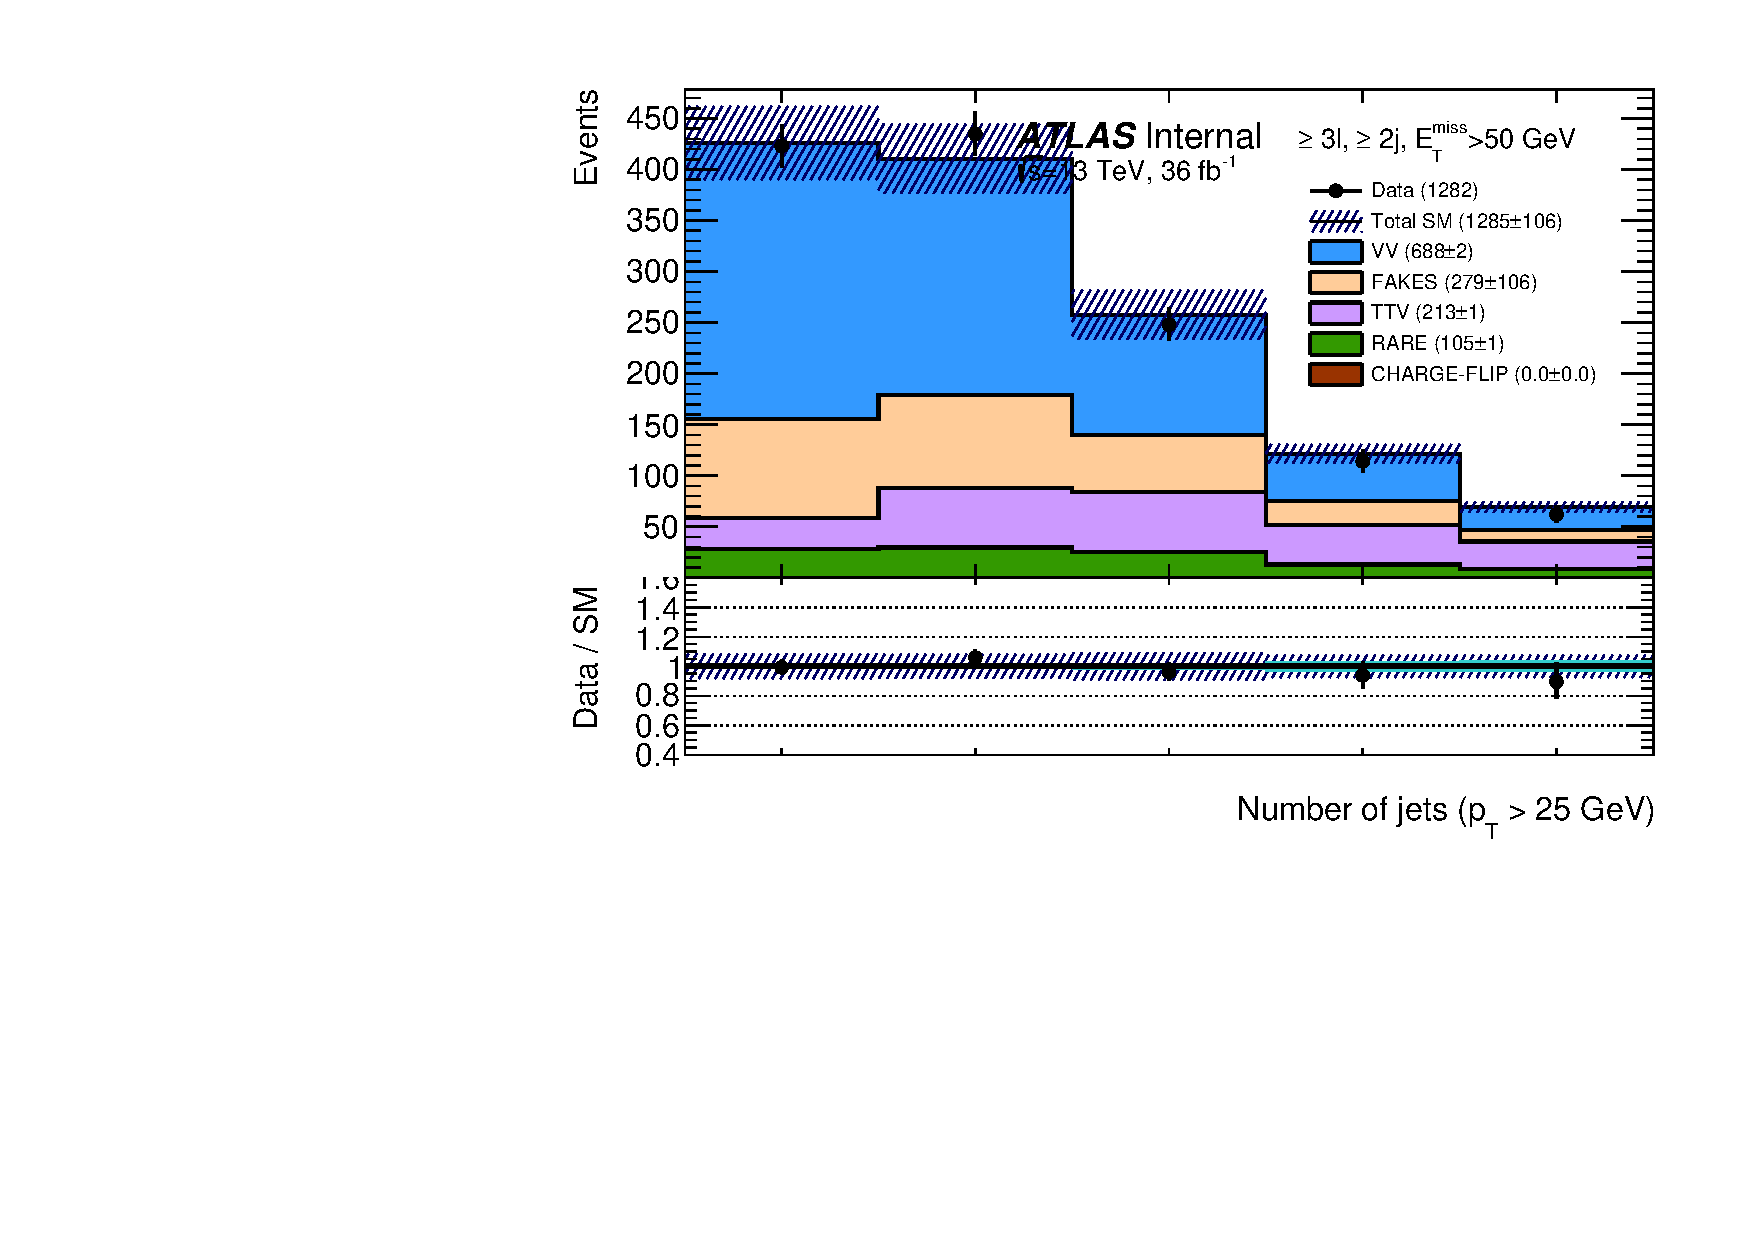
\includegraphics[width=\textwidth]{TRILEP_2JMET50_njets25}
\caption{Number of jets ($\pt>25~\GeV$)}
\end{subfigure}
\begin{subfigure}[t]{0.48\textwidth}
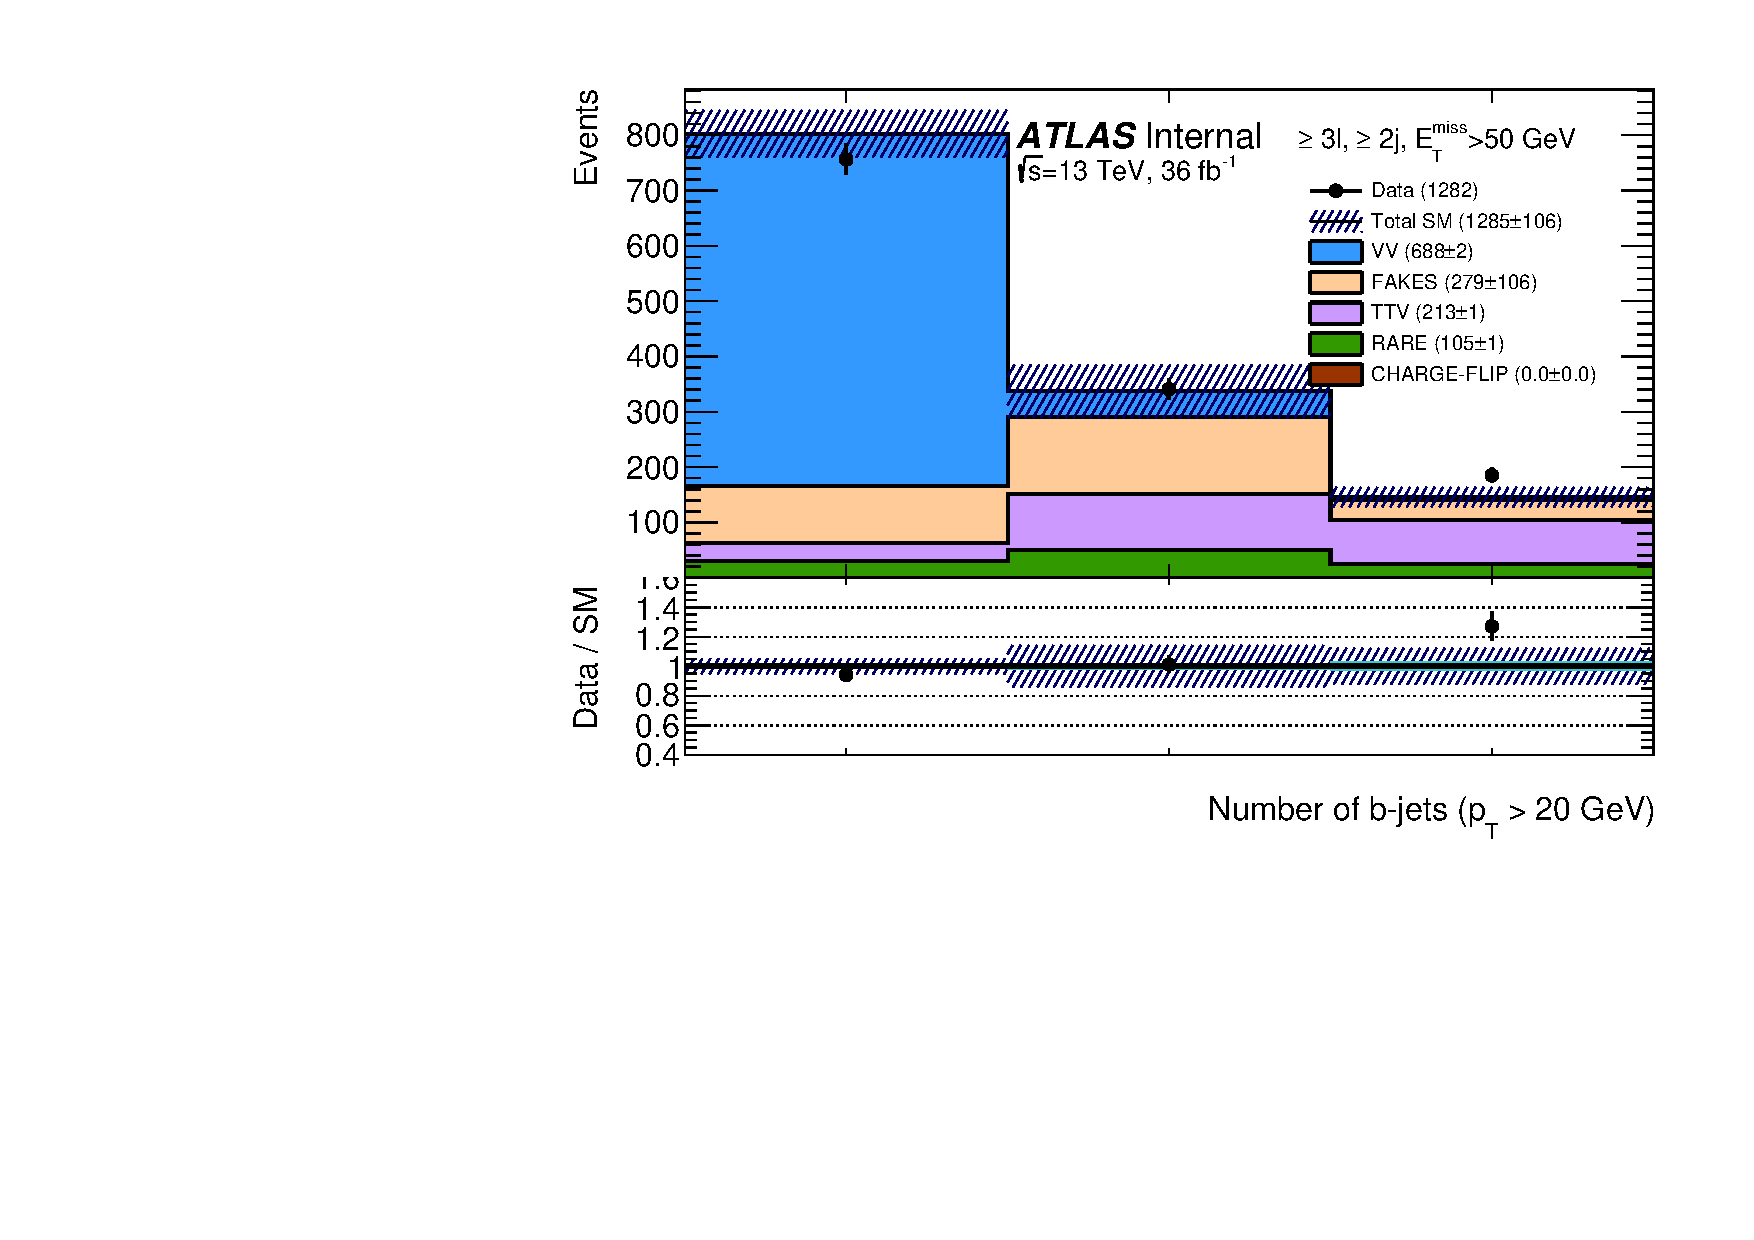
\includegraphics[width=\textwidth]{TRILEP_2JMET50_nbjets}
\caption{Number of $b$-tagged jets ($\pt>20~\GeV$)}
\end{subfigure}
\begin{subfigure}[t]{0.48\textwidth}
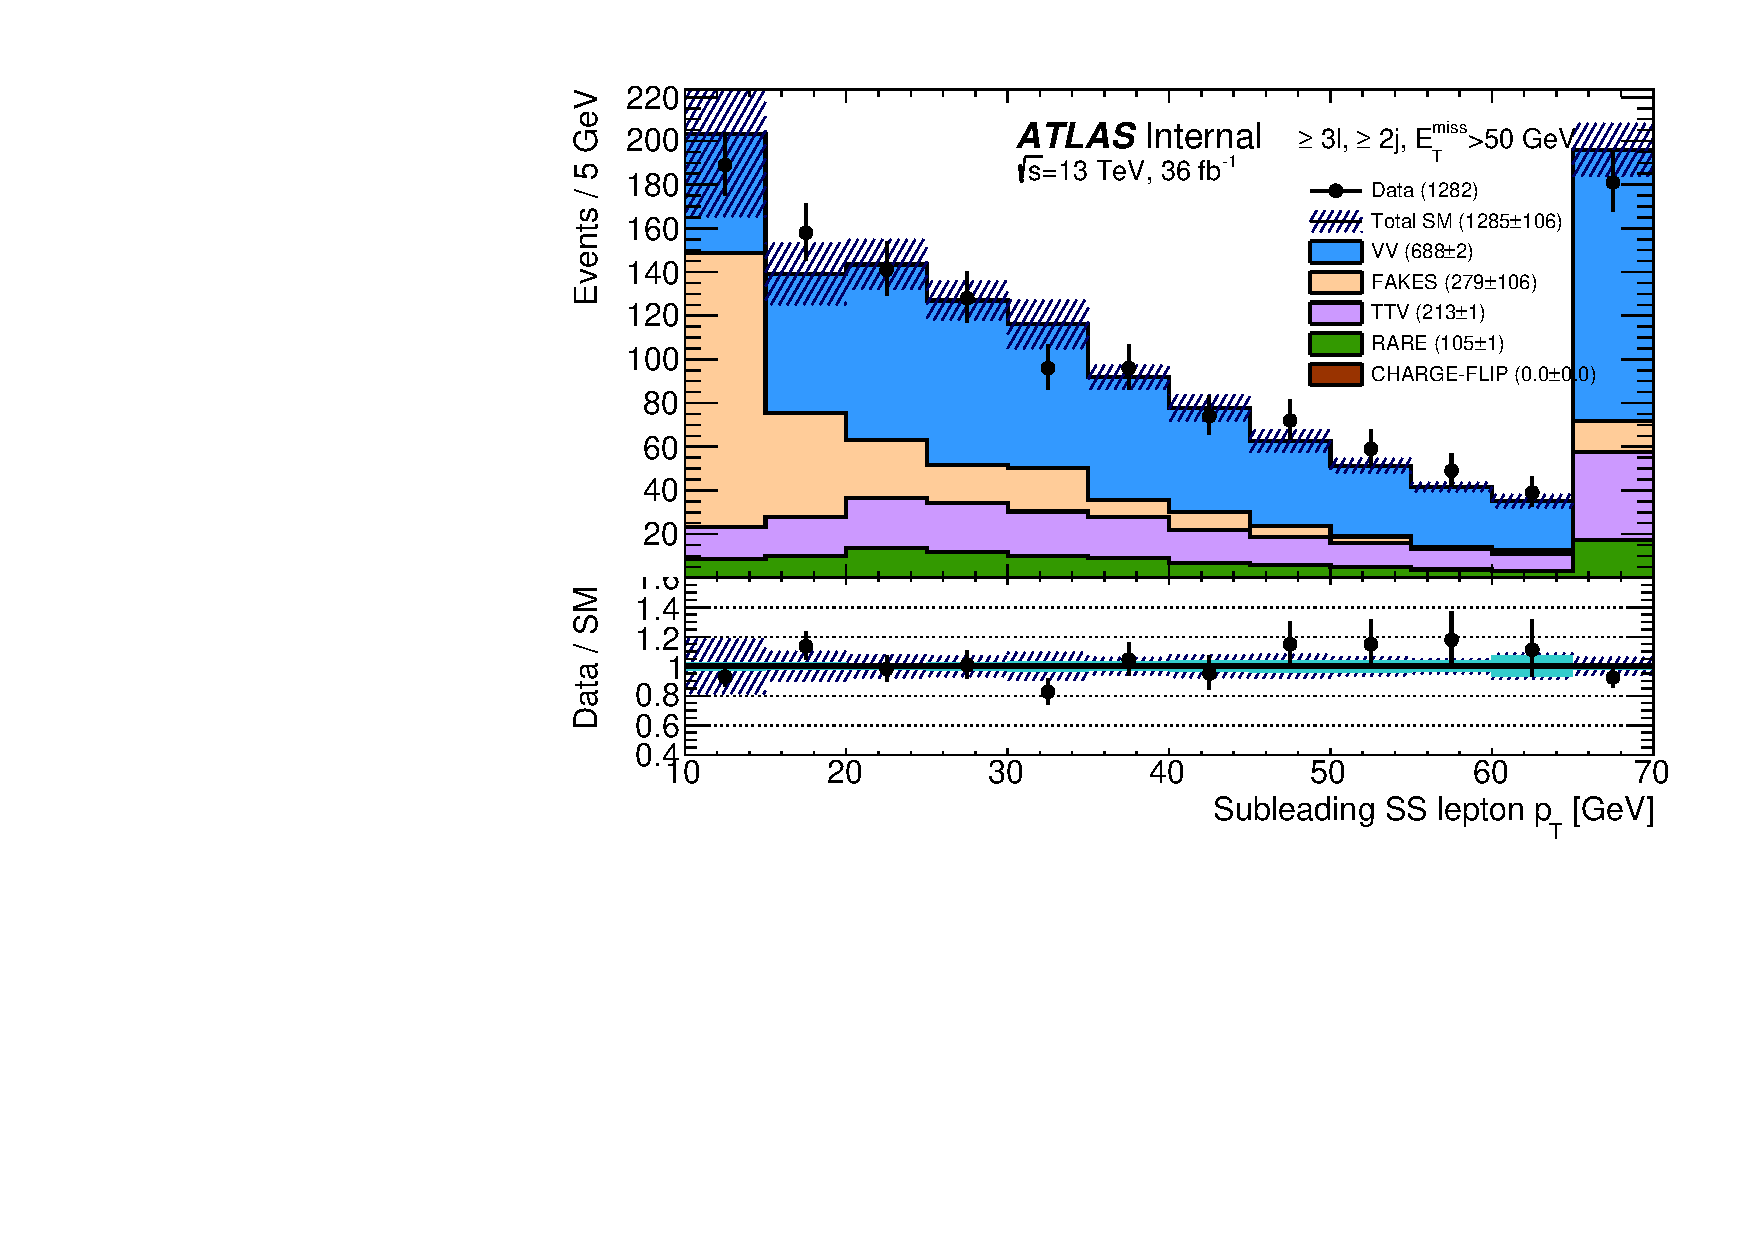
\includegraphics[width=\textwidth]{TRILEP_2JMET50_subSS_Pt}
\caption{Subleading SS lepton \pt}
\end{subfigure}
\caption{Trilepton channel: comparisons between observed data (2015+2016, 36 \ifb) and expected SM+detector backgrounds 
for events with $\ge 3$ leptons ($\pt>20~\GeV$ for the two leading leptons, $\pt>10~\GeV$ for the third lepton), $\met>50~\GeV$ and $\ge 2$ jets ($\pt>40~\GeV$). 
Uncertainties include statistical sources, as well as systematic uncertainties for the data-driven backgrounds; 
for illustration, statistical uncertainties alone are shown in the light-colored error bands in the ratio plots. 
Events belonging to any of the signal regions are rejected, both in data and MC.  
}
\label{fig:distributions_channel3L_2015}
\end{figure} 
